%% appendix
\section{Cavity stability criteria ($G(g_1,g_2)$)} \label{sec:cavstab}
Using spherical mirror resonators to match the phasefront of the beam mode is a standard practice that has some additional geometric considerations to maximize reonance for a given beam. Choosing two mirrors with ROCs ($R_1$, $R_2$) and a set distance between them $d$, a implicit containment condition is set on the resonator \cite{salehteich:2007}:

$$
	0 \leq \bigg(1 + \frac{d}{R_1} \bigg) \bigg(1 + \frac{d}{R_2} \bigg) \leq 1
$$

Where we define $g_i = 1 + \frac{d}{R_i}$ so that we define a single parameter for the two mirror resonator $G$:

\begin{equation}\label{eq:cavstab}
	0 \leq G(g_1,g_2) \leq 1
\end{equation}

\begin{figure}[H]
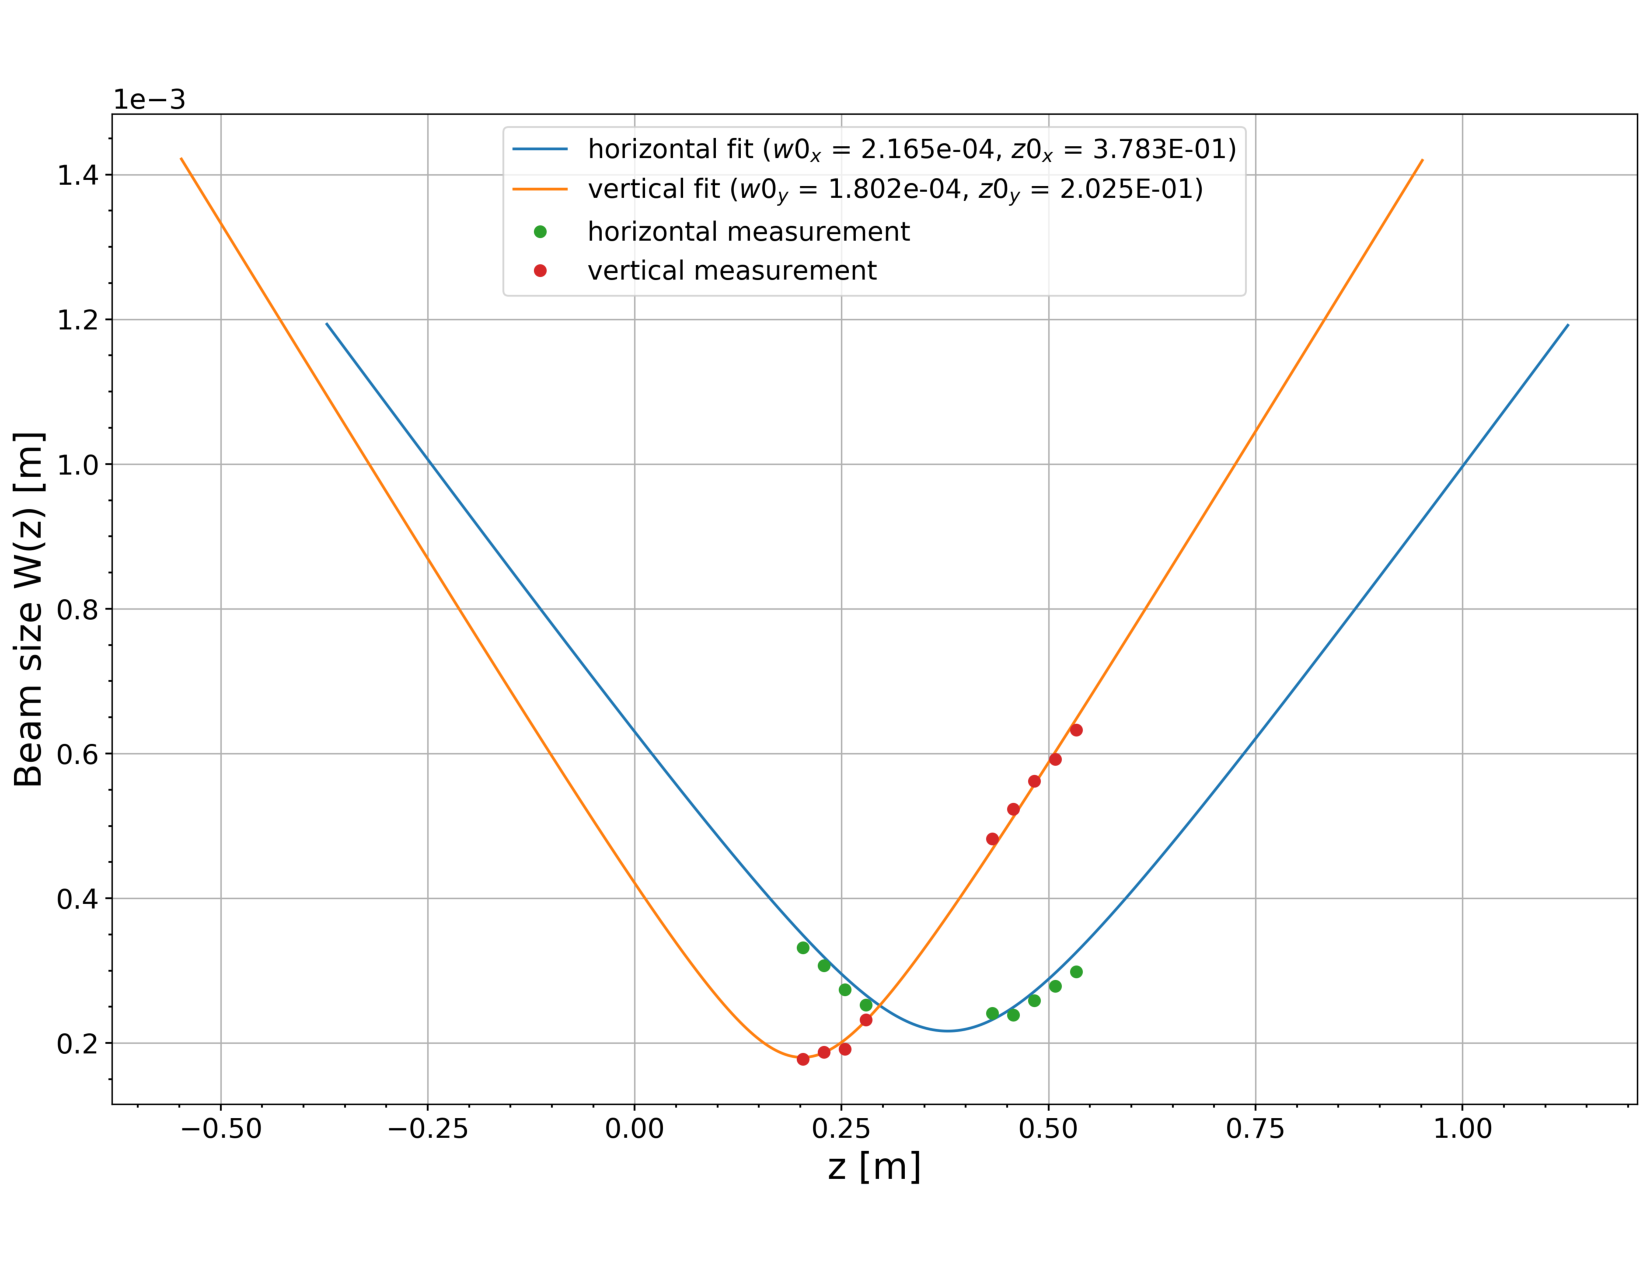
\includegraphics[width=\textwidth]{figs/ALGAAS/beam_scans/12_18_2020_preMMT.pdf}
\caption{\textcolor{red}{Figure of two mirror cavity}}
\label{fig:cav_stab}
\end{figure}

\section{Paraxial equation} \label{sec:paraxial}

The general three dimensional wave equation for an E-field $E(x,y,z,t)$ is provided by Maxwell:

$$ \label{eq:waveq}
	\bigg( \nabla ^2 + \frac{1}{c^2} \frac{\partial^2}{\partial t^2} \bigg) E(x,y,z,t) = 0
$$

For a coherent beam ($k = \frac{2 \pi}{\lambda}$), we analyze the purely spatial component of the solution and select a longitudinal propogation ($\vec{z}$) direction such that our solution will look like the following (utilizing Helmholtz's equation):

$$
	E(x,y,z) = E_0(x,y,z) e^{-ikz}
$$

The above wavefunction combined with Helmoltz equation requires that complex form of $E_0$ obeys the paraxial equation:

\begin{equation}\label{eq:paraxial}
	\bigg( \frac{\partial^2}{\partial x ^2} + \frac{\partial^2}{\partial y^2} - 2ik \frac{\partial}{\partial z} \bigg) E_0(x,y,z) = 0
\end{equation}

\section{The Equipartition theorem and the Fluctuation dissapation theorem}

\section{Monochromatic plane wave propogation}
Revisiting Maxwell's equations for a simple monochromatic plane wave solution provides further direction on how crystalline media may effect incident light. Further elaborating, the following assumptions are made:
\begin{equation}
\vec{E} = E_o e^{(i \omega (\frac{n}{c} \vec{r}\cdot \vec{s}-t))}
\end{equation}
Where $n$ is the index of refraction, $c$ is the speed of light, $\vec{r}$ is the position vector and $\vec{s}$ is the unit wave normal.
\begin{equation}
\nabla \times \vec{H}= \frac{\partial \vec{D}}{\partial t}
\end{equation}
Where $\vec{H}$ is the magnetic field assuming permeability $\mu$, and the generalized displacement vector $\vec{D}$ and electric field vector $\vec{E}$.
\begin{equation}
\nabla \times \vec{E} = -\mu \vec{H}
\end{equation}
Reducing to only the displacement and electric fields:
\begin{equation}\label{eq:dispelec}
\vec{D} = \frac{n^2}{\mu}[\vec{E}-\vec{s}(\vec{s}\cdot \vec{E})]
\end{equation}
Maxwell's equations show that the electric field is not necessarily parallel to the displacement field and in most materials with non-zero polarizability tensors and dielectric tensors, it is not. But as specified above, the displacement vector, Electric field and unit wave normal are co-planar while remaining orthogonal to $\vec{H}$. Assuming we are operating within a coordinate system aligned with the principal dielectric axes, we substitute \autoref{eq:dispfield} into \autoref{eq:dispelec}:
\begin{equation}
E_i = \frac{n^2 s_i (\vec{E}\cdot\vec{s})}{n^2 - \mu \varepsilon_i}
\end{equation}

From here it can be shown that for a general plane wave there exist two unique refractive index solutions within the constructed dielectric ~\cite{nye}. 

\newpage

\section{Thermo-optic filters}\label{sec:TO_filt}

\subsection{COMSOL self heating filter}
\begin{figure}[H]
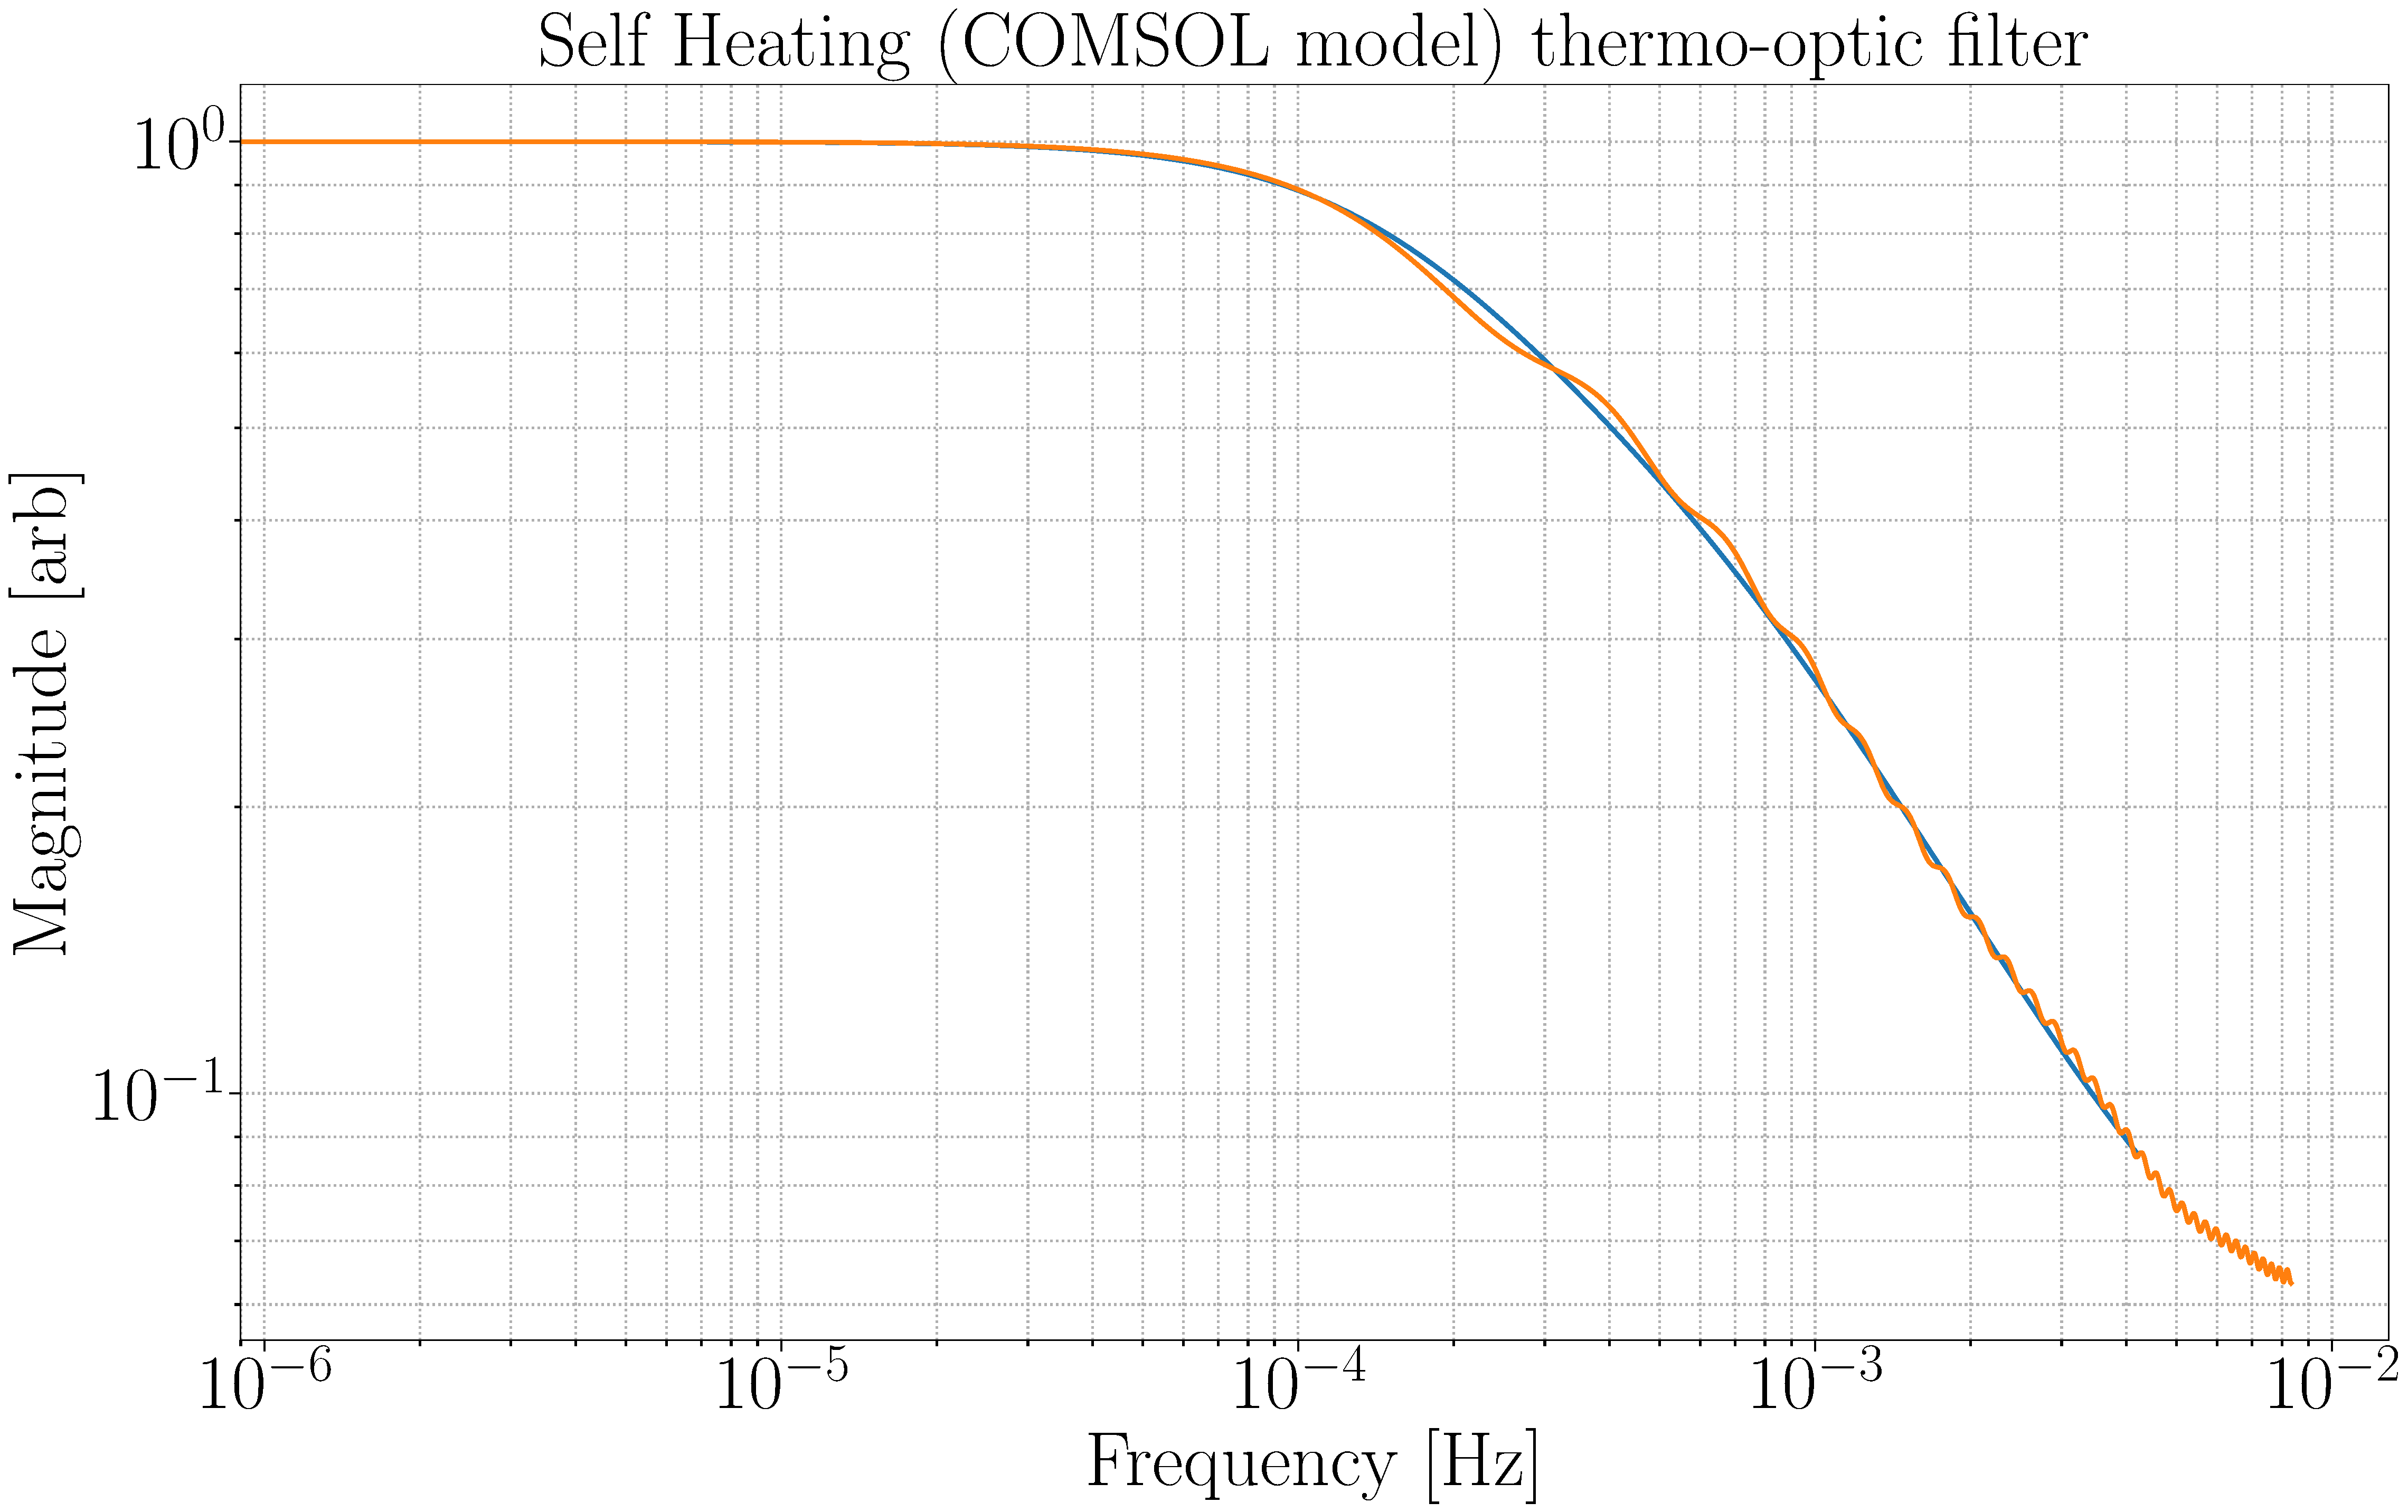
\includegraphics[width=\textwidth]{figs/TCS/self_heating_zpk.pdf}
\caption{Fitted zpk filter to transient response of self heating COMSOL model.}
\label{fig:self_zpk_fit}
\end{figure}

\subsection{RH filter}


\subsection{CO2 filter}
\begin{figure}[H]
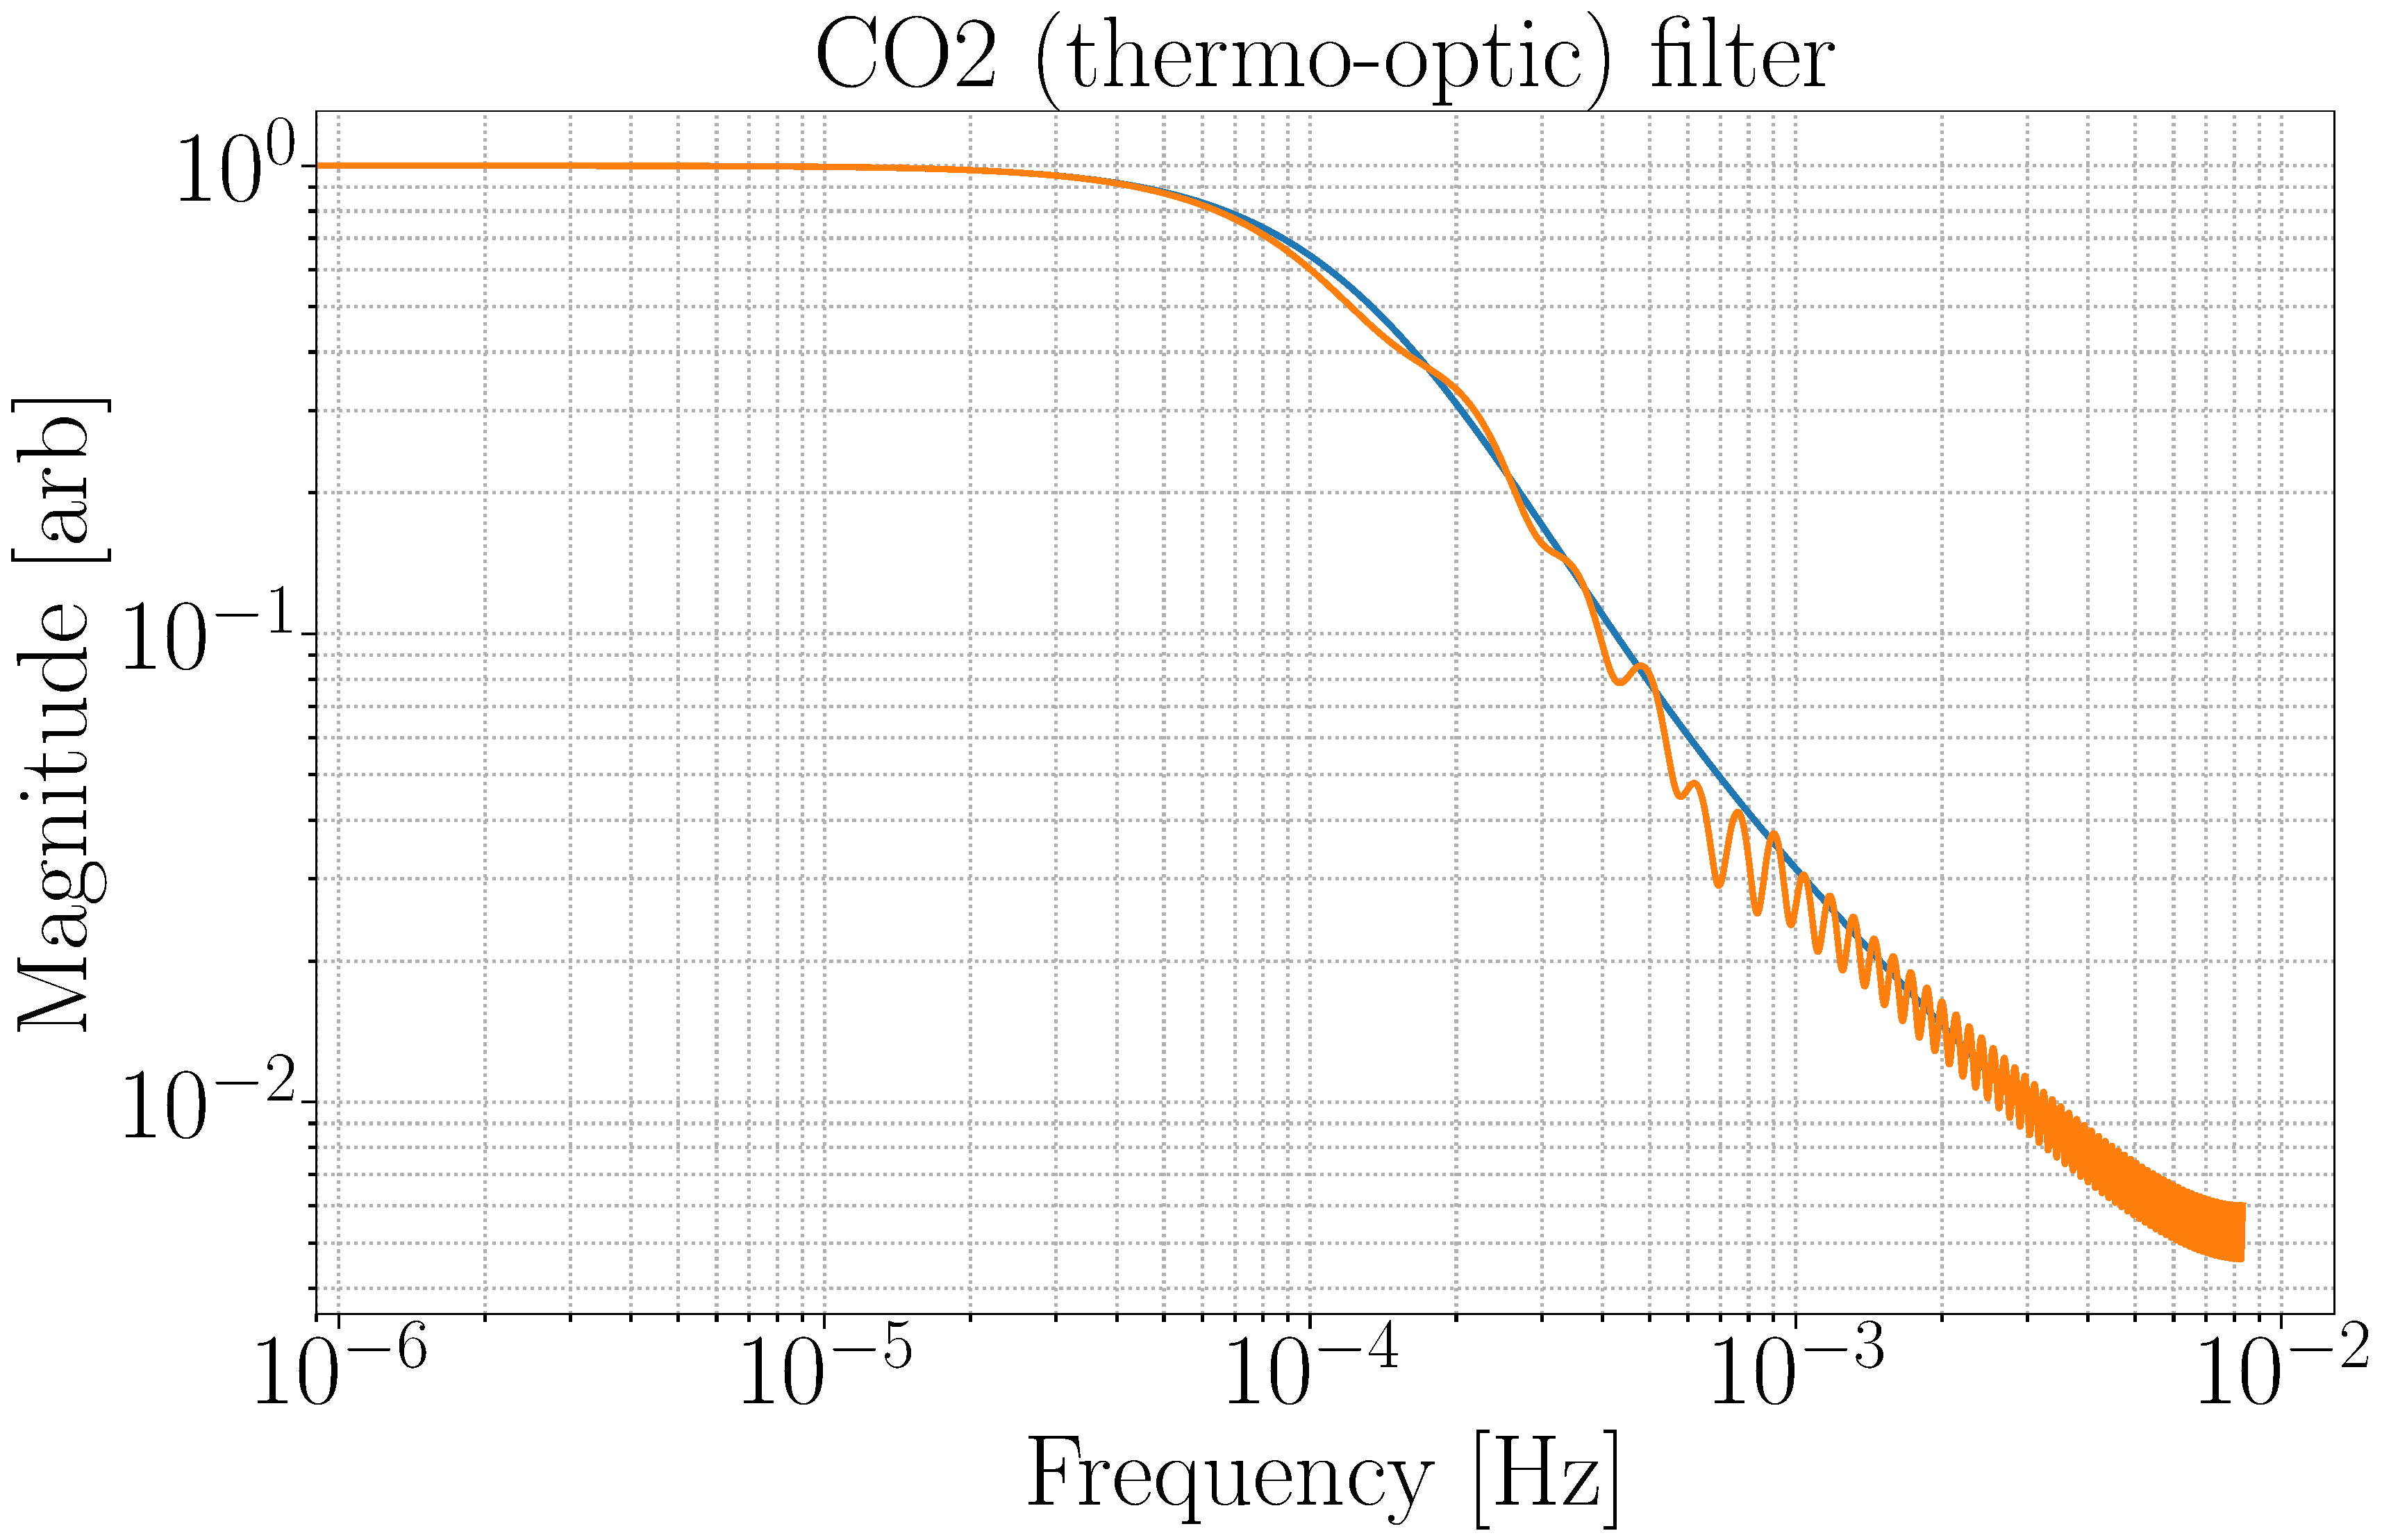
\includegraphics[width=\textwidth]{figs/TCS/CO2_zpk.pdf}
\caption{Fitted zpk filter to transient CO2 actuation response.}
\label{fig:co2_zpk_fit}
\end{figure}

\subsection{Transient RH thermo-optic response}

\begin{equation}
	\Psi(t,r)=2\frac{dn}{dT} \sum^{\infty}_{m,p = 1} A_{m,p} \; c^{u}_{p} \mathrm{sin}(u_m h /2a) (a/u_m)[1-e^{-\alpha t}] J_0(\zeta_p r/a)
\end{equation}

\subsection{Conditioned RH input filter}
\begin{enumerate}	
	\item Fit step response to a zpk filter $H(s)$ 
	\item Invert fitted filter ($H(s) \rightarrow H^{-1}(s)$) 
	\item Apply correction filter $G(s)$ for stability and speed tuning ($H^{-1}(s)*G(s)$)
\end{enumerate}

\section{Mode matching data for Electro-optic sample cavity}

\subsection{Pre MMT beam scan}

\begin{figure}[H]
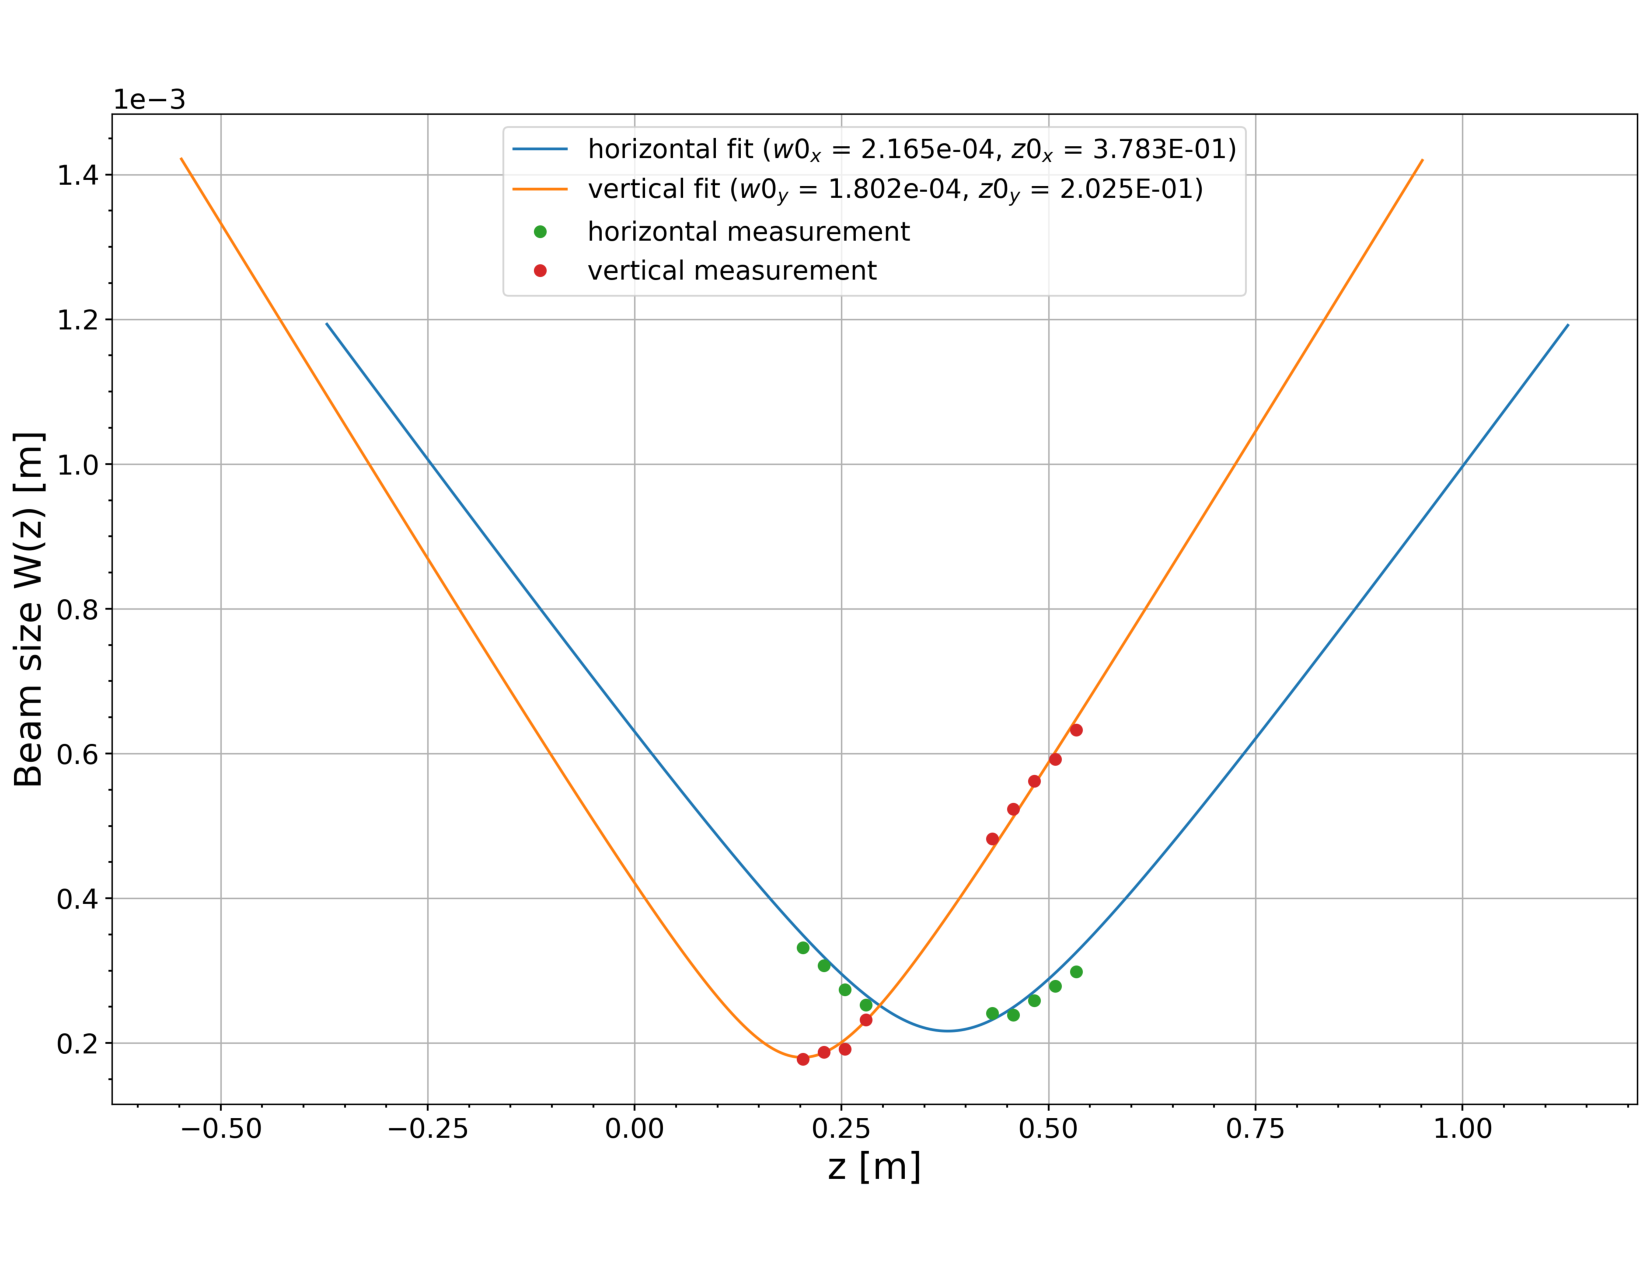
\includegraphics[width=\textwidth]{figs/ALGAAS/beam_scans/12_18_2020_preMMT.pdf}
\caption{Beam scan taken from SM5 (Steering mirror 5)}
\label{fig:beamscan2020}
\end{figure}


\subsection{``Just another mode matching tool" (JAMMT) solution}
\subsection{Post MMT beam scan}

\begin{figure}[H]
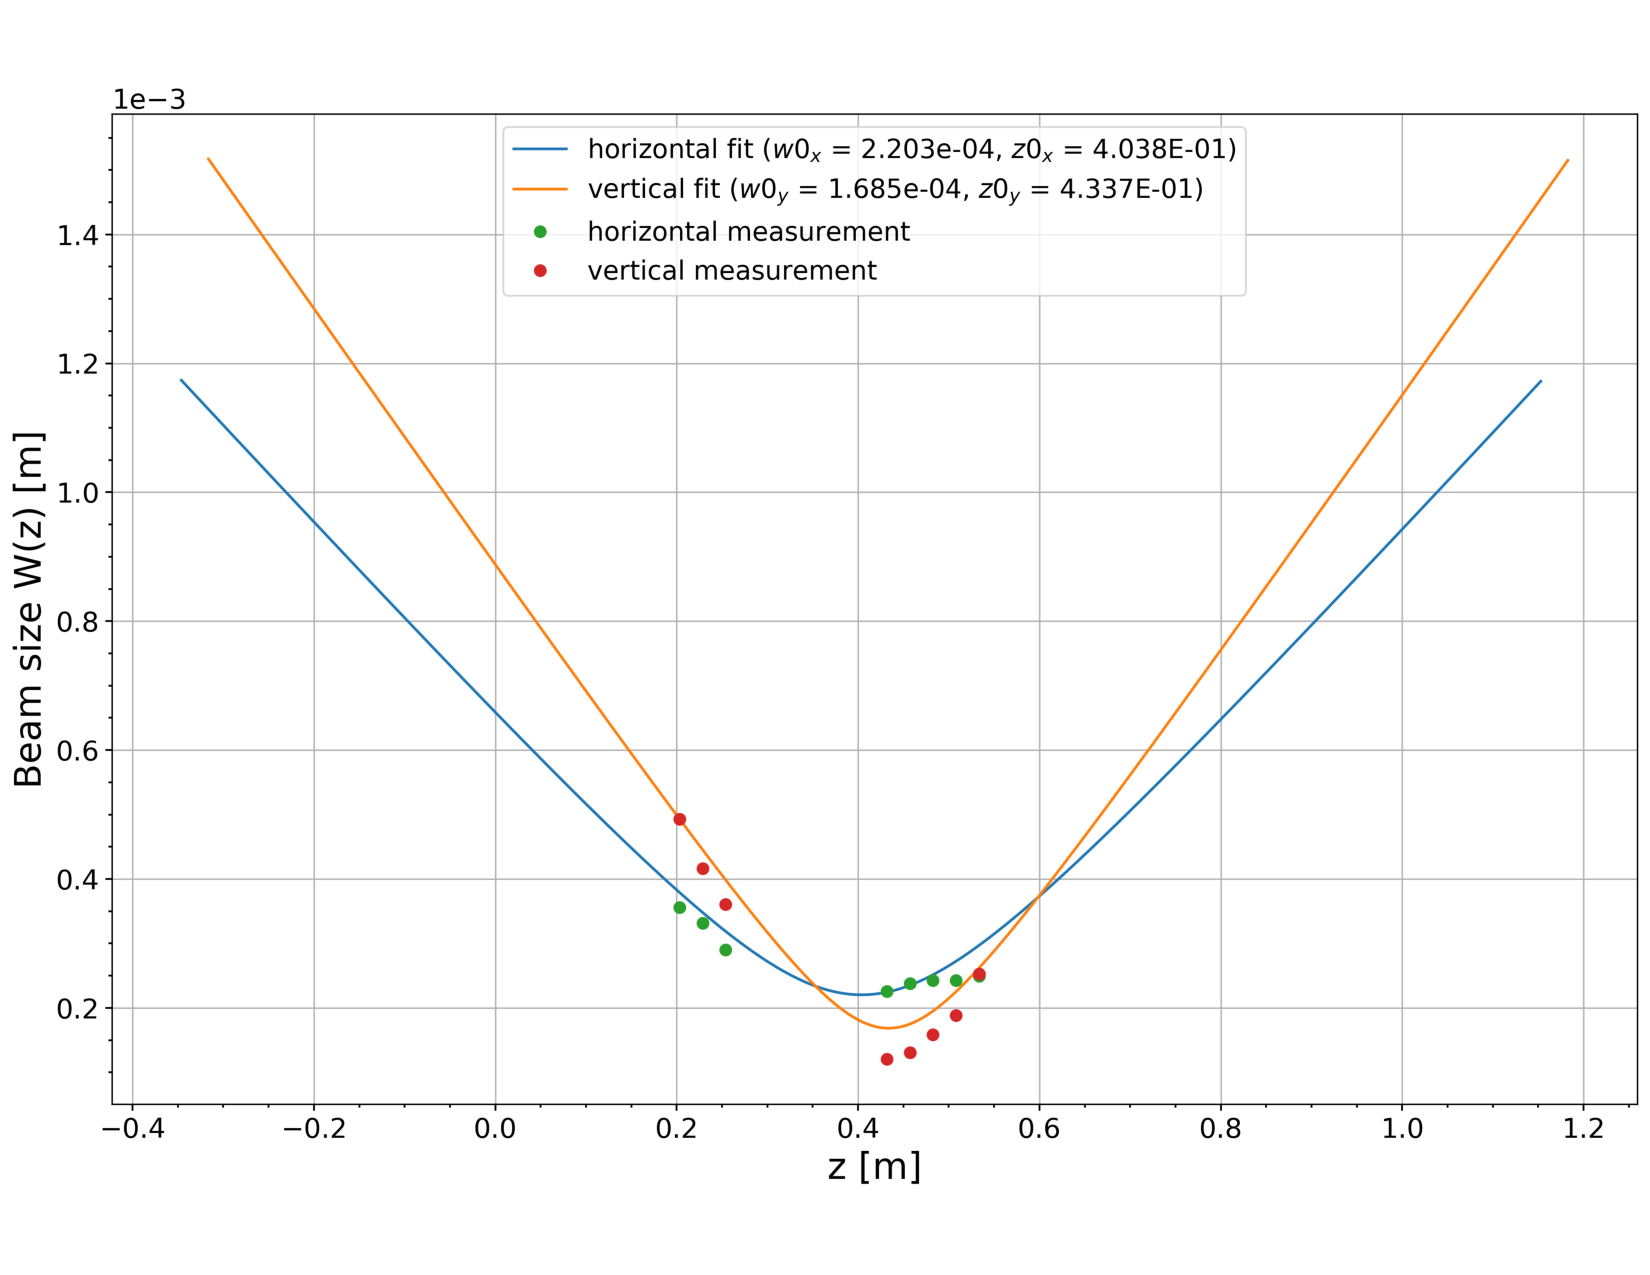
\includegraphics[width=\textwidth]{figs/ALGAAS/beam_scans/01_12_2021_postMMT.pdf}
\caption{Beam scan taken from SM6. Sampling points before SM7 and after the first cavity iris.}
\label{fig:beamscan2021}
\end{figure}

\subsection{Laser PZT sweep}

\begin{figure}[H]
	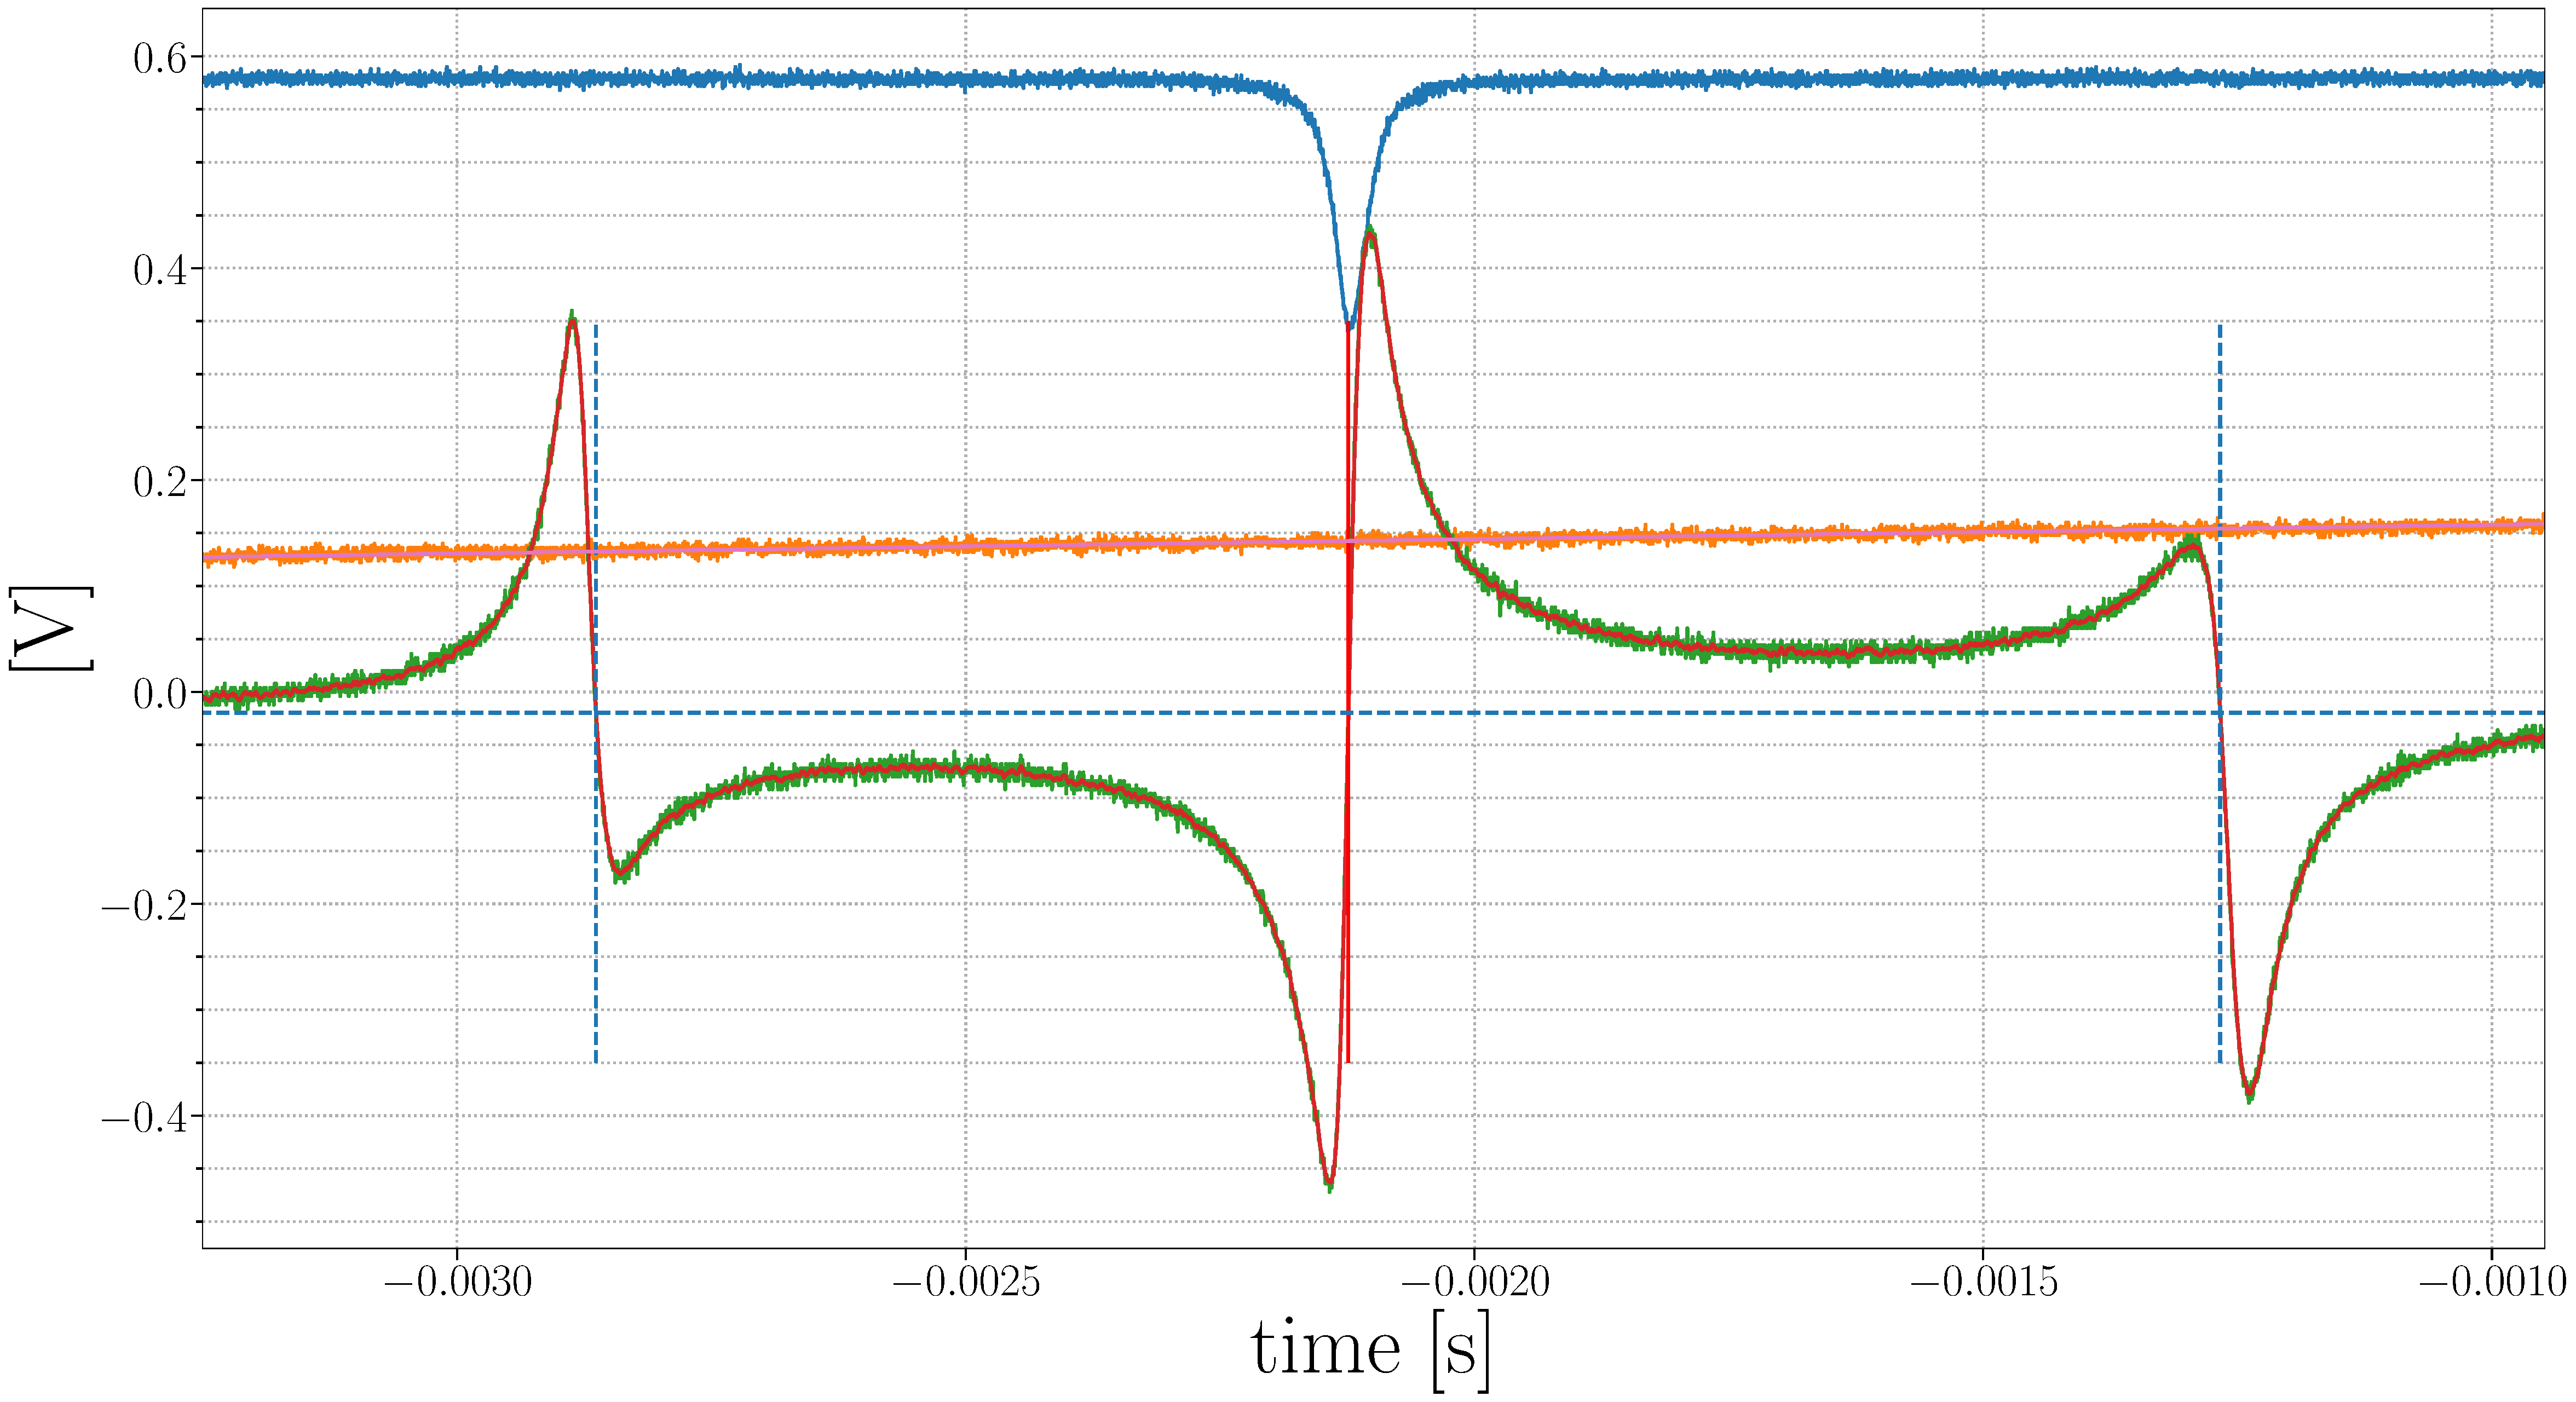
\includegraphics[width=\textwidth]{figs/ALGAAS/pdh_measured.pdf}
	\caption{Ramping voltage sent to the laser PZT while probing the mixer output. The sweep was performed for sample cavity of length notes}
\label{fig:pdhmeasured}
\end{figure}

\newpage

\section{Assembly blueprints and alternative views}

\subsection{Assembly 1}

\subsubsection{Cross section}

\subsubsection{Electrodes}

\subsubsection{Iteration 1.1}

\begin{figure}[!ht]
	\begin{subcaptiongroup}
		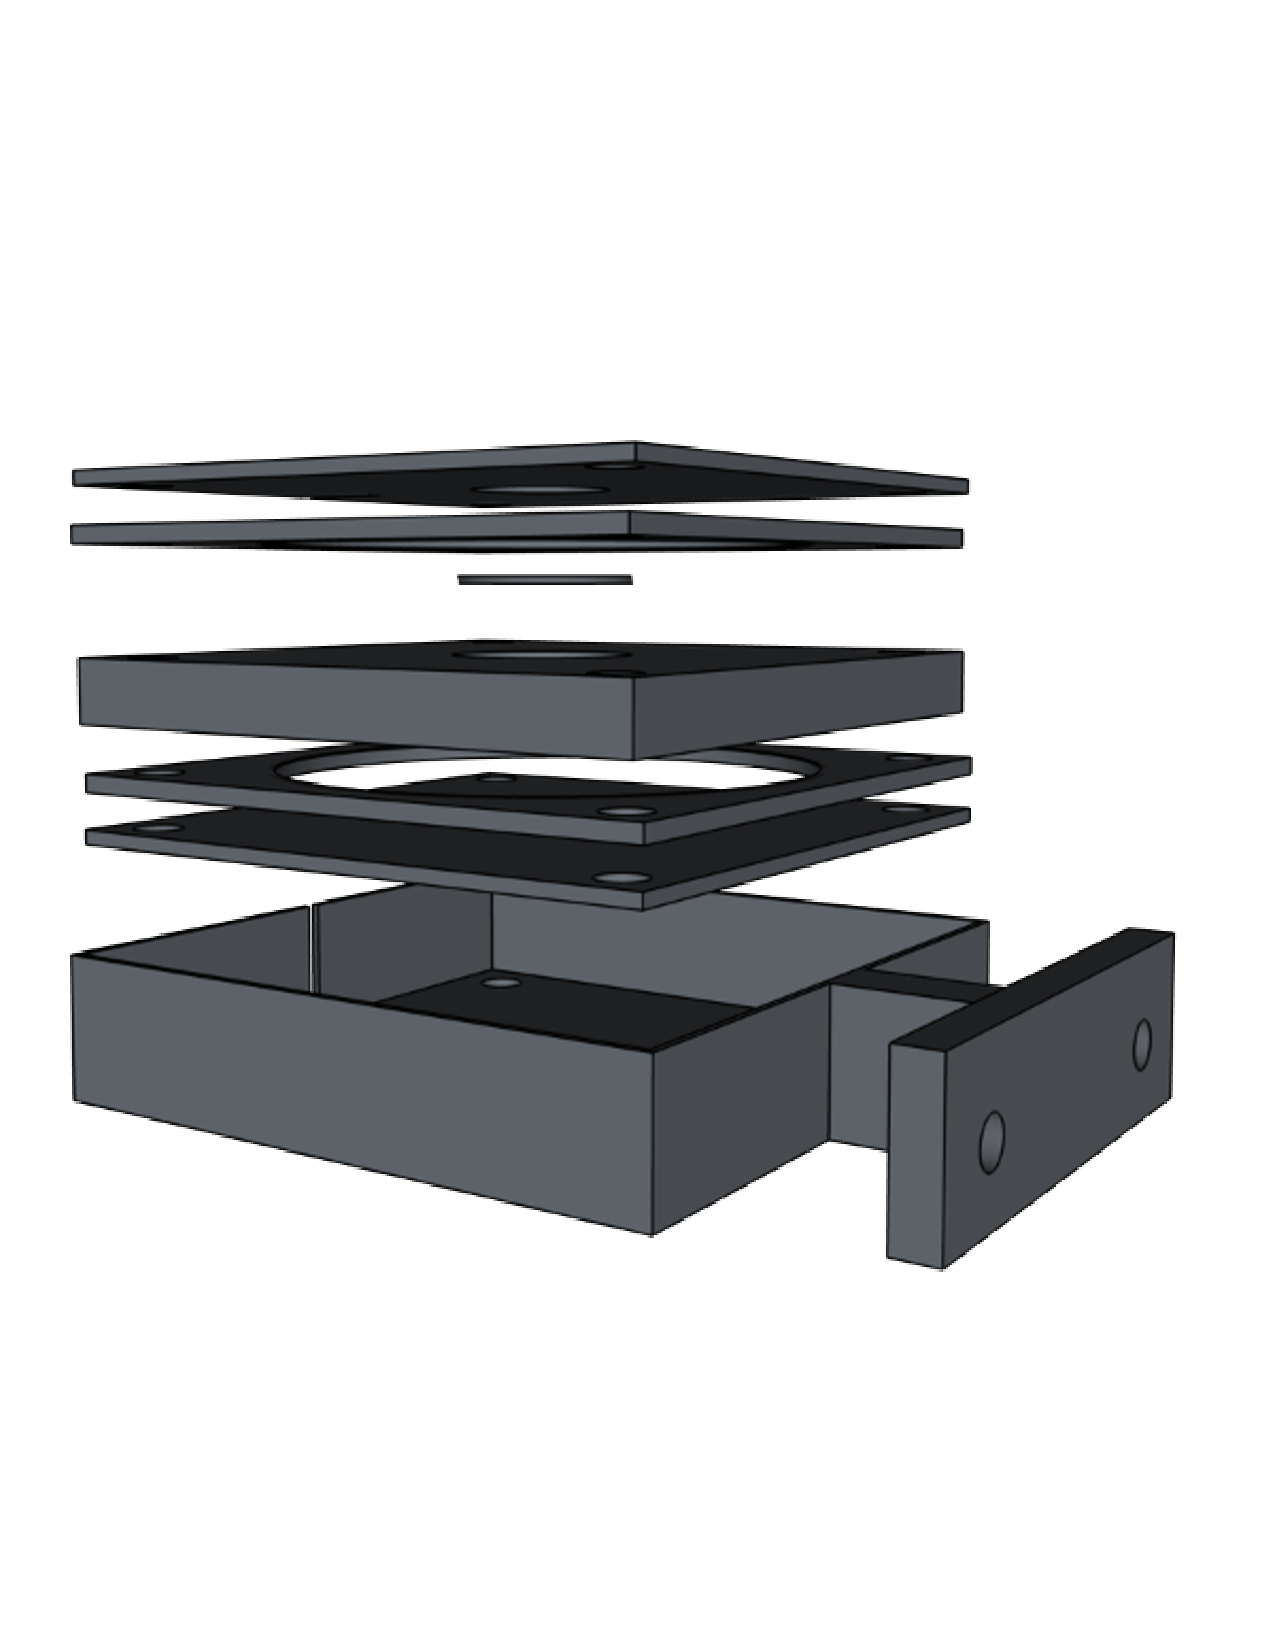
\includegraphics[width=.5\textwidth]{figs/ALGAAS/assemblies/assembly0/assembly0.pdf}
		\phantomcaption\label{A0}
		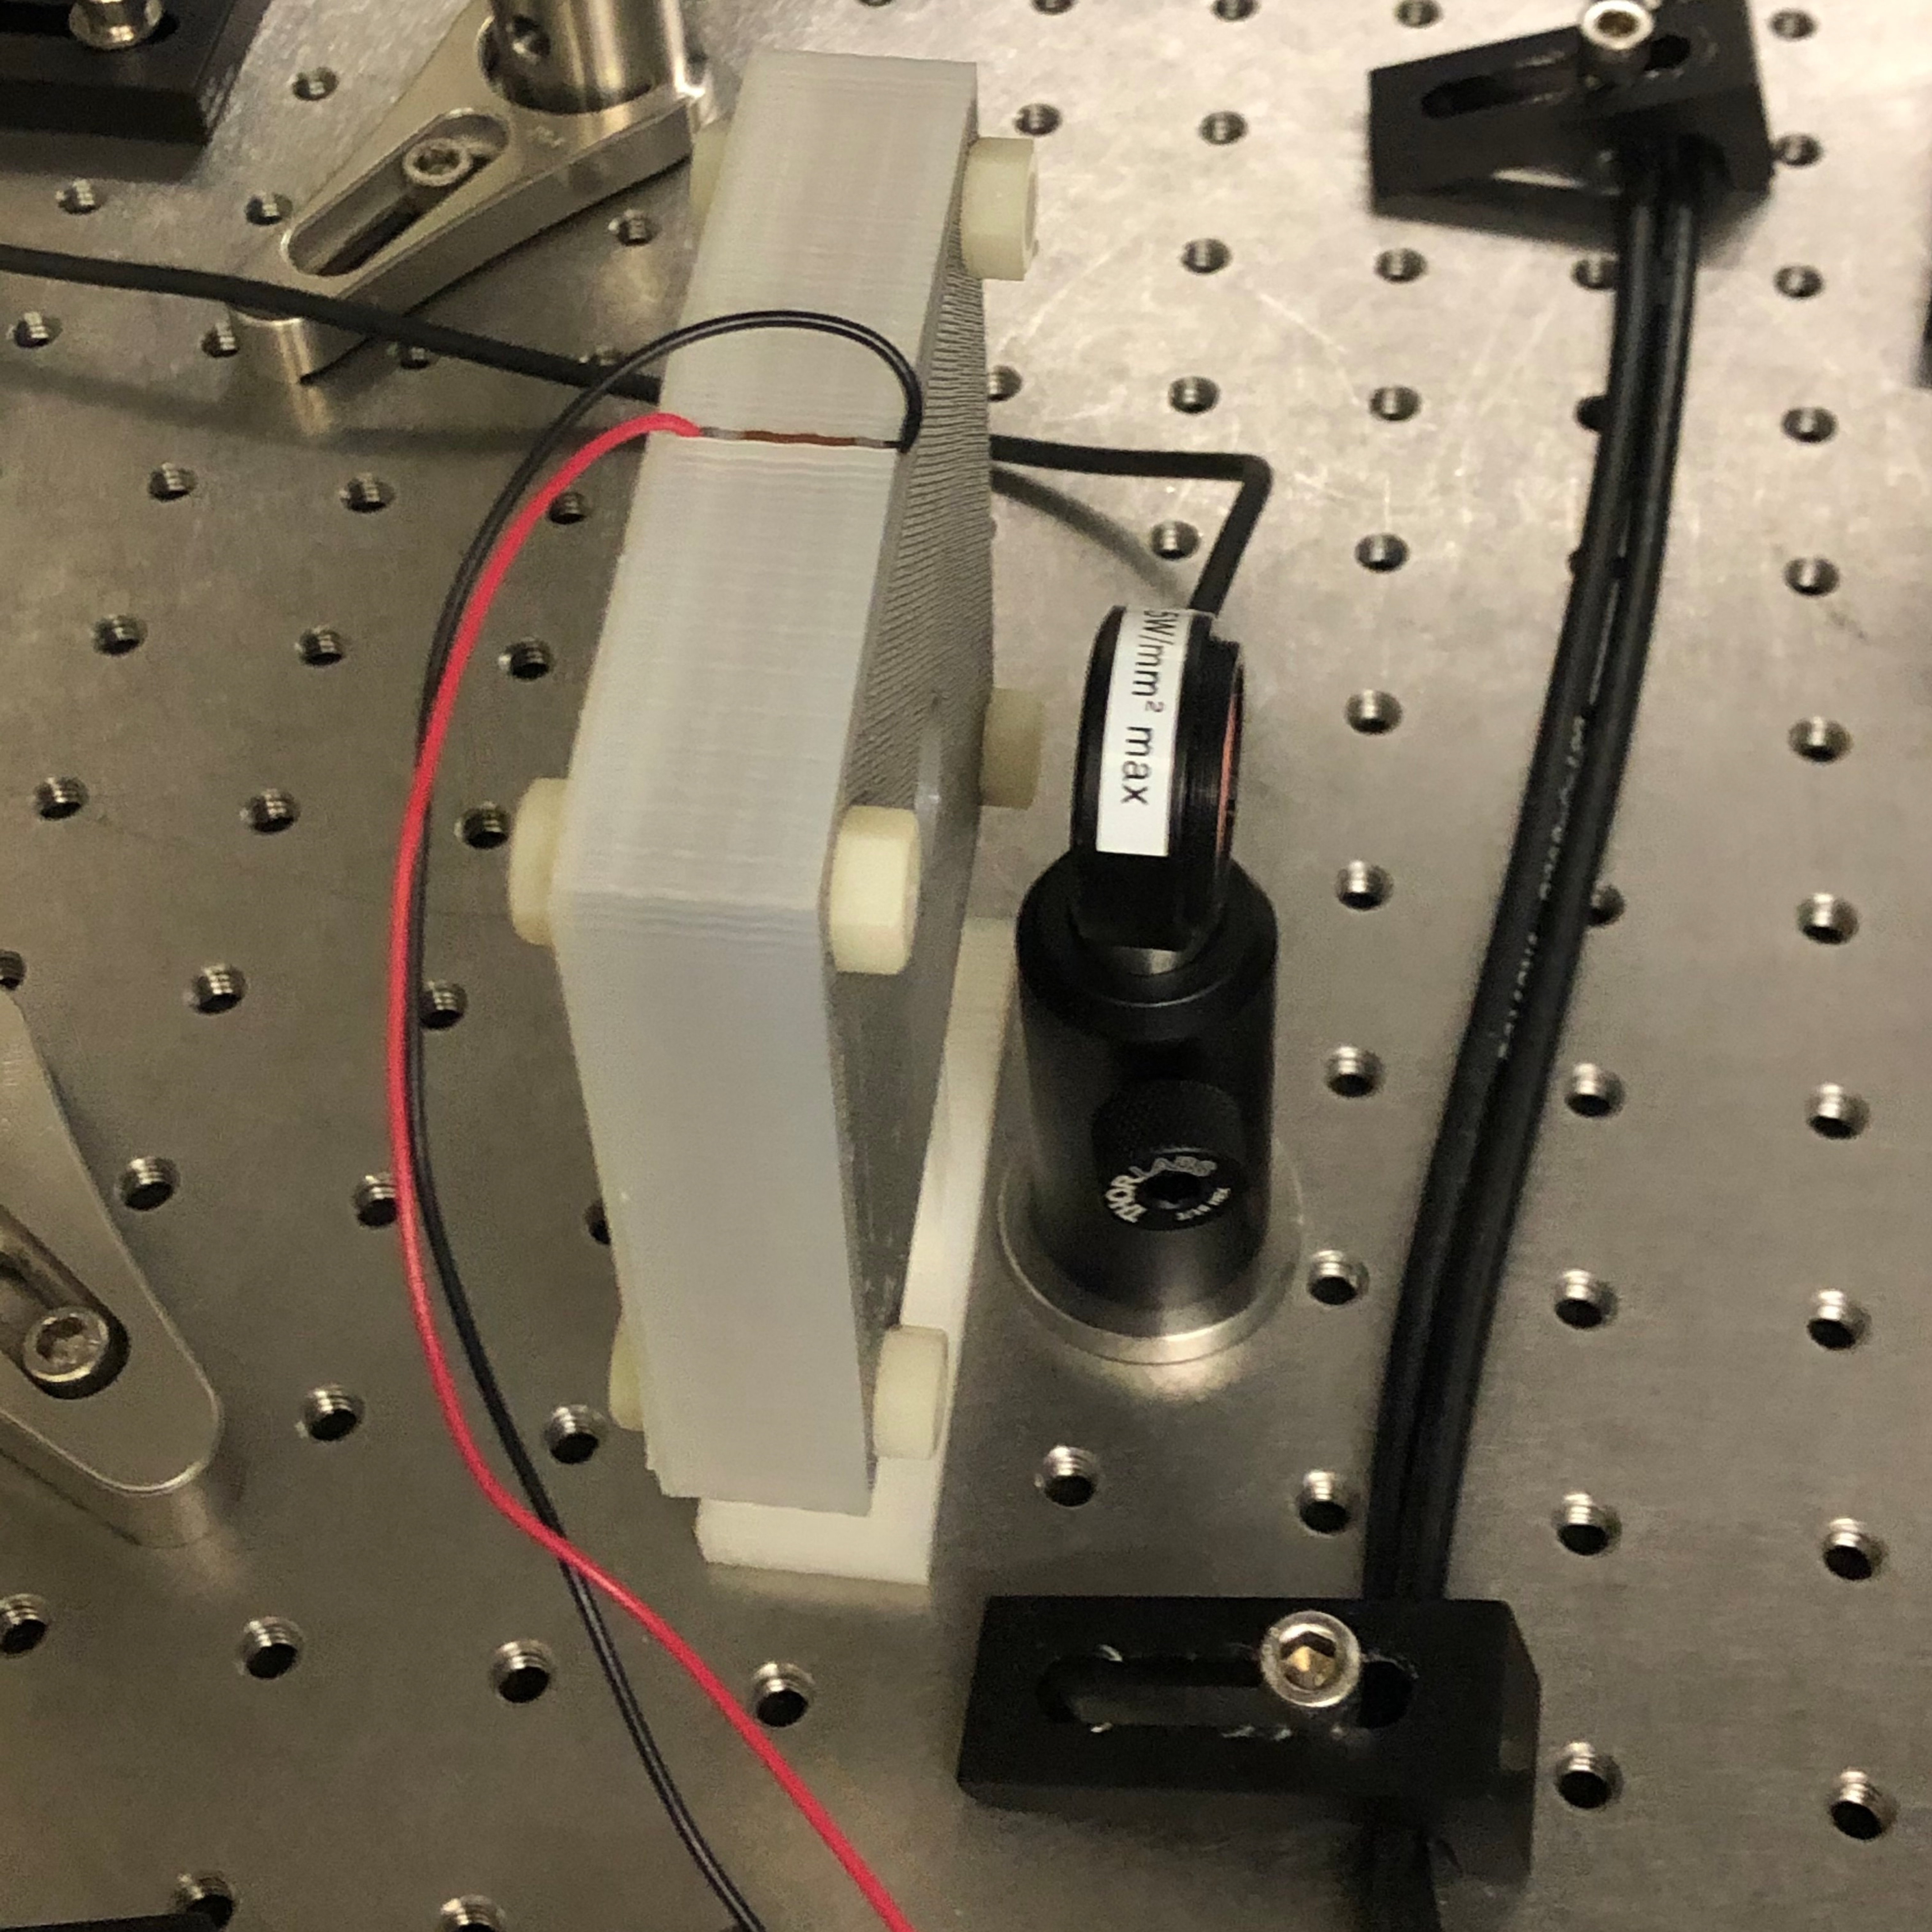
\includegraphics[width=.5\textwidth]{figs/ALGAAS/assemblies/assembly0/assembly0_incident_power.pdf}
 		\phantomcaption\label{A0inc}
	\end{subcaptiongroup}
  \caption{Assembly 0 was constructed to meet the criteria of providing a non-conductive housing for the electrode / sample assembly while maintaining a fixed length spacing using parts 3d printed with polylactic acid (PLA).}
  \label{fig:assembly0bp}
\end{figure}
\FloatBarrier

\subsubsection{Iteration 1.2}
\begin{figure}[!ht]
	\begin{subcaptiongroup}
		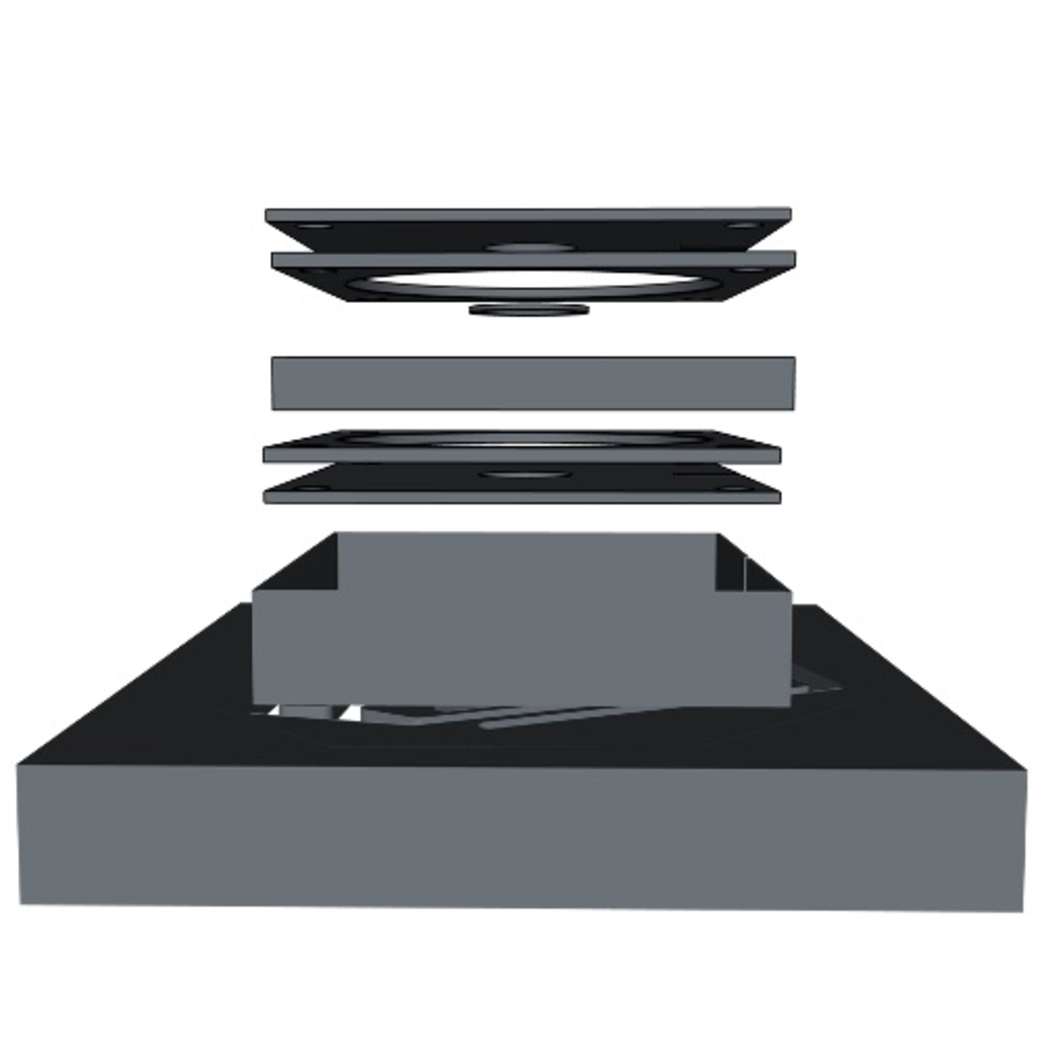
\includegraphics[width=.5\textwidth]{figs/ALGAAS/assemblies/assembly1/assembly1_dissassembled.pdf}
		\phantomcaption\label{A1pt2CAD}
		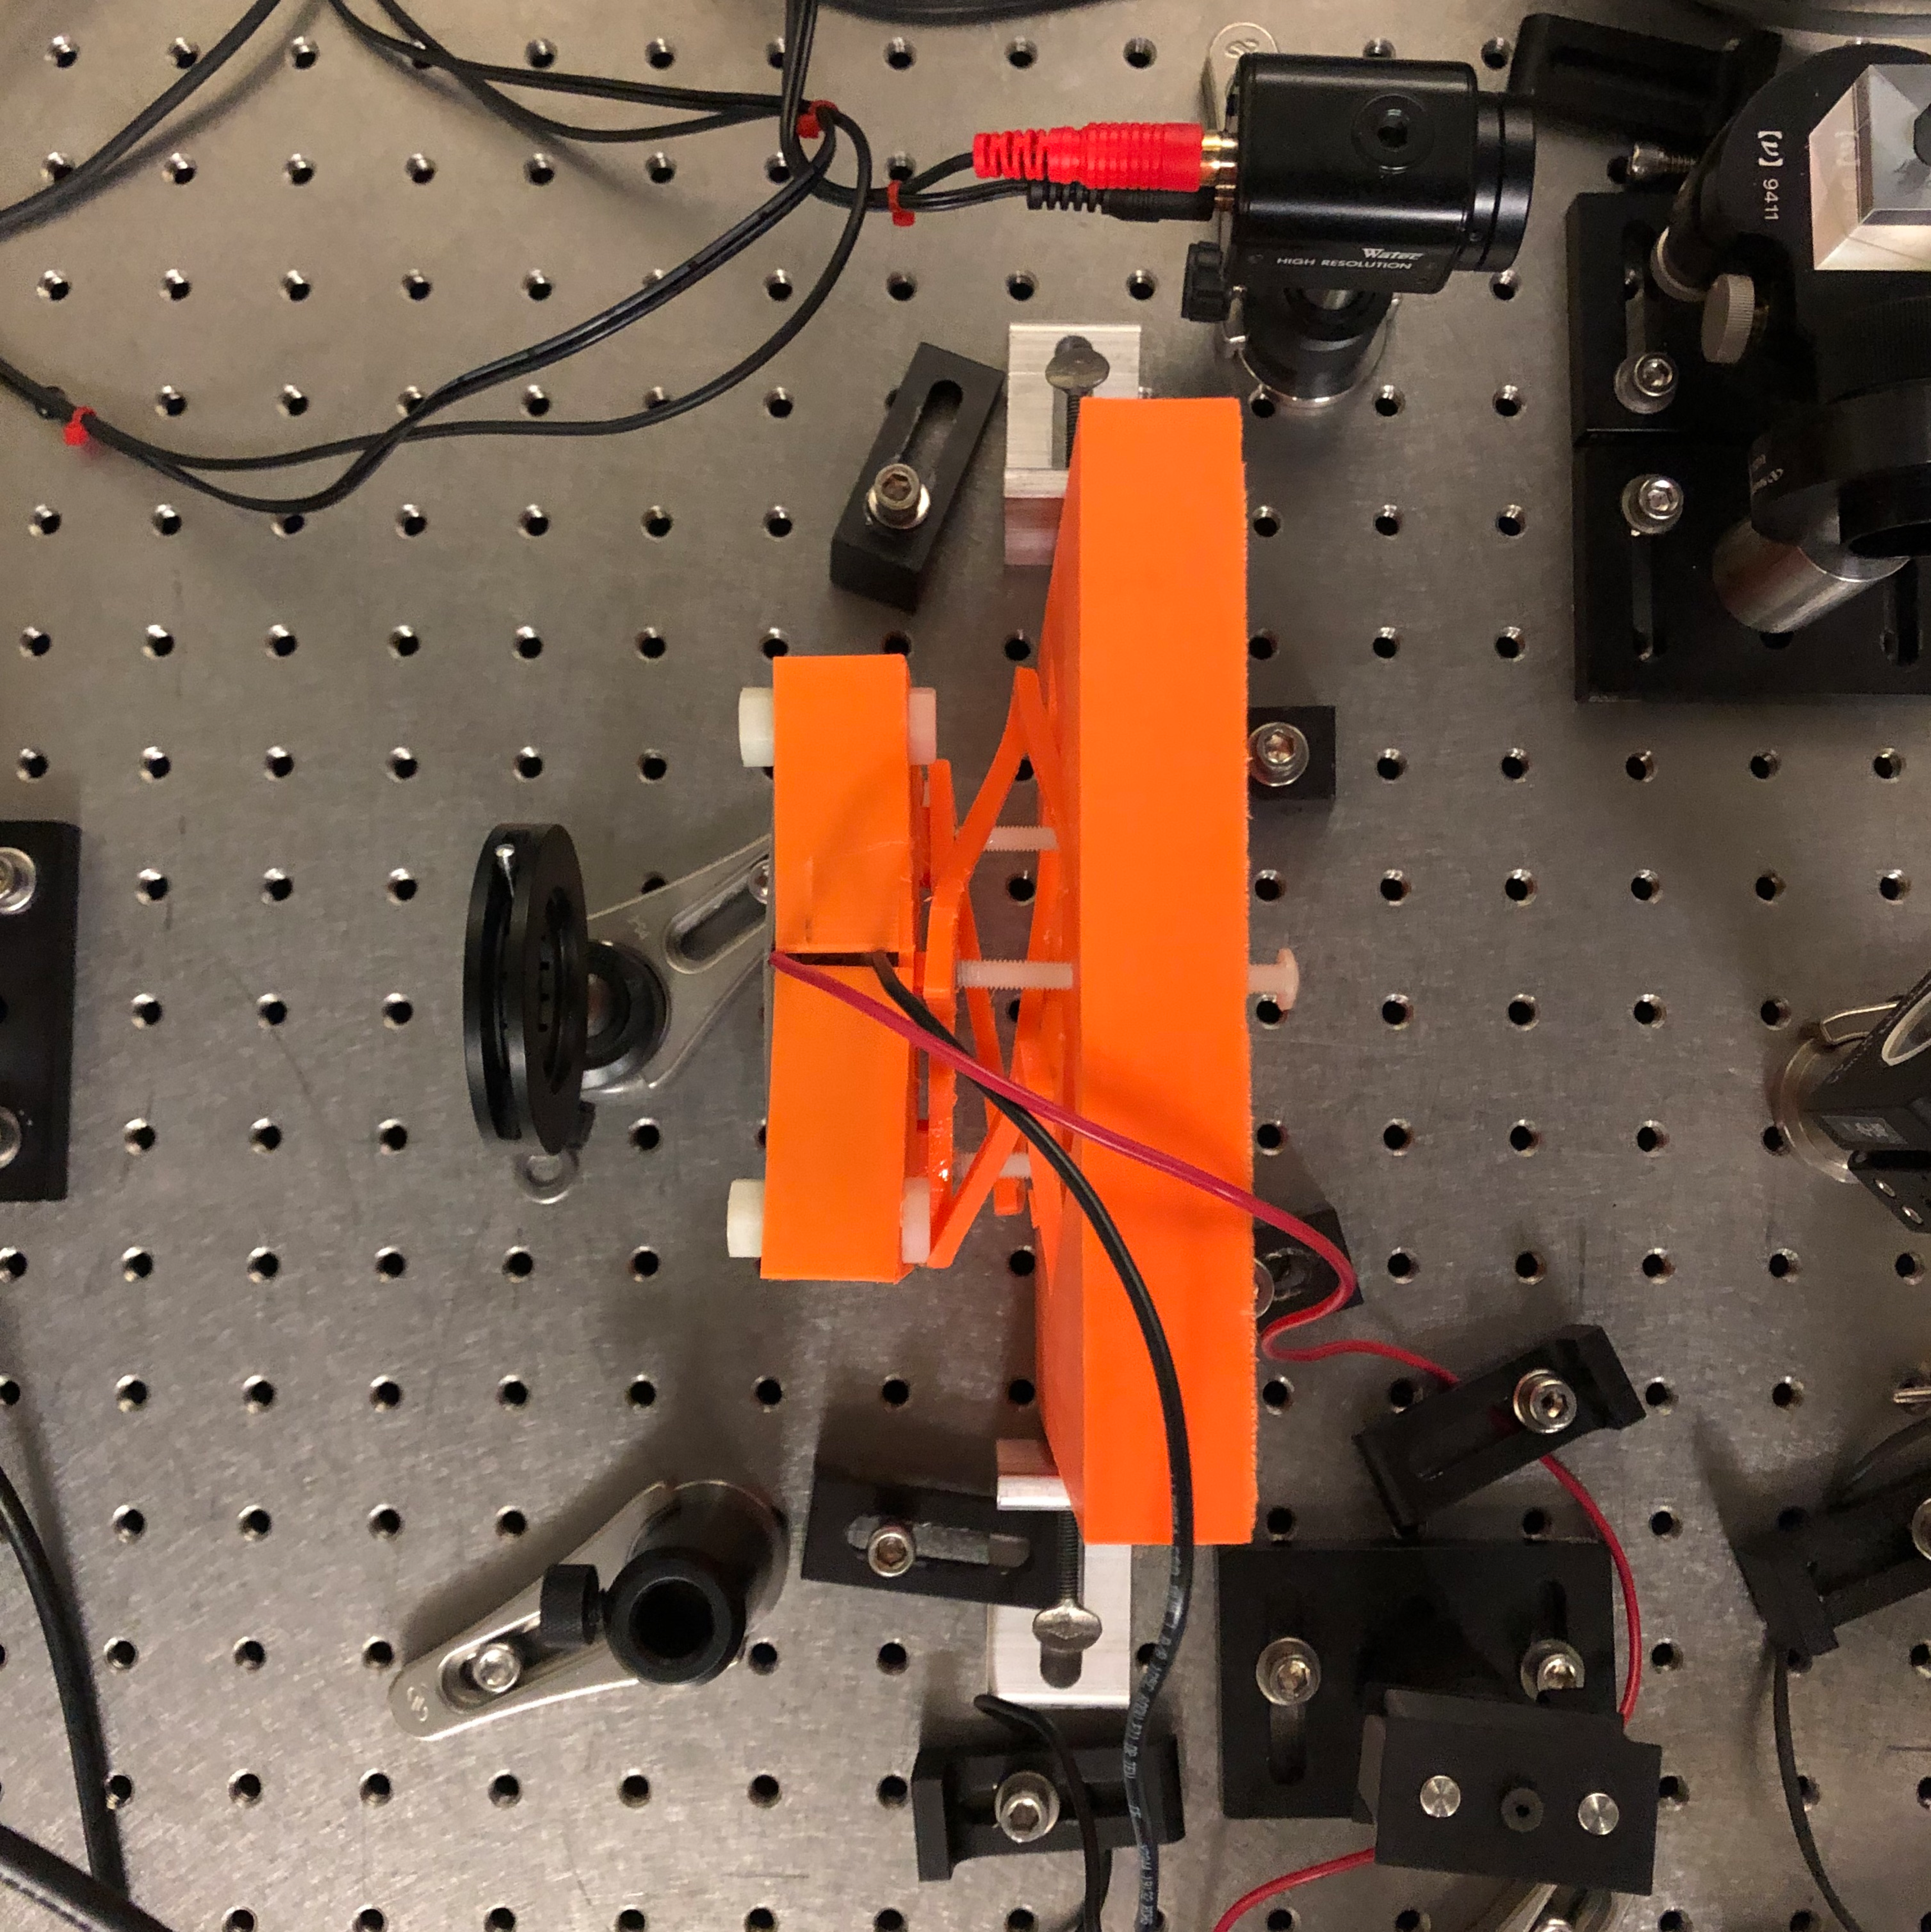
\includegraphics[width=.5\textwidth]{figs/ALGAAS/assemblies/assembly1/assembly1_insitu2.pdf}
		\phantomcaption\label{A1pt2pic}	
	\end{subcaptiongroup}
	\caption{Assembly 1 was constructed to meet the criteria of providing a non-conductive housing for the electrode / sample assembly while maintaining a fixed length spacing using parts 3d printed with polylactic acid (PLA).}
	\label{fig:assembly1bp}
\end{figure}
\FloatBarrier

\subsubsection{Iteration 1.3}
\begin{figure}[!ht]
	\begin{subcaptiongroup}
		\includegraphics[width=.5\textwidth]{figs/ALGAAS/assemblies/assembly1/assembly1_mod_front.pdf}
		\phantomcaption\label{A1pt3CAD}
		\includegraphics[width=.5\textwidth]{figs/ALGAAS/assemblies/assembly1/assembly1_mod_side.pdf}
		\phantomcaption\label{A1pt3pic}
	\end{subcaptiongroup}
	\caption{A modification implemented with the intention of reducing pitch dithering while still having control of DC YAW}
	\label{fig:assembly1mod}
\end{figure}

\newpage

\subsection{Assembly 2}
\subsubsection{Cross section}

\subsubsection{Electrodes}

\begin{figure}[H]
  \centering
  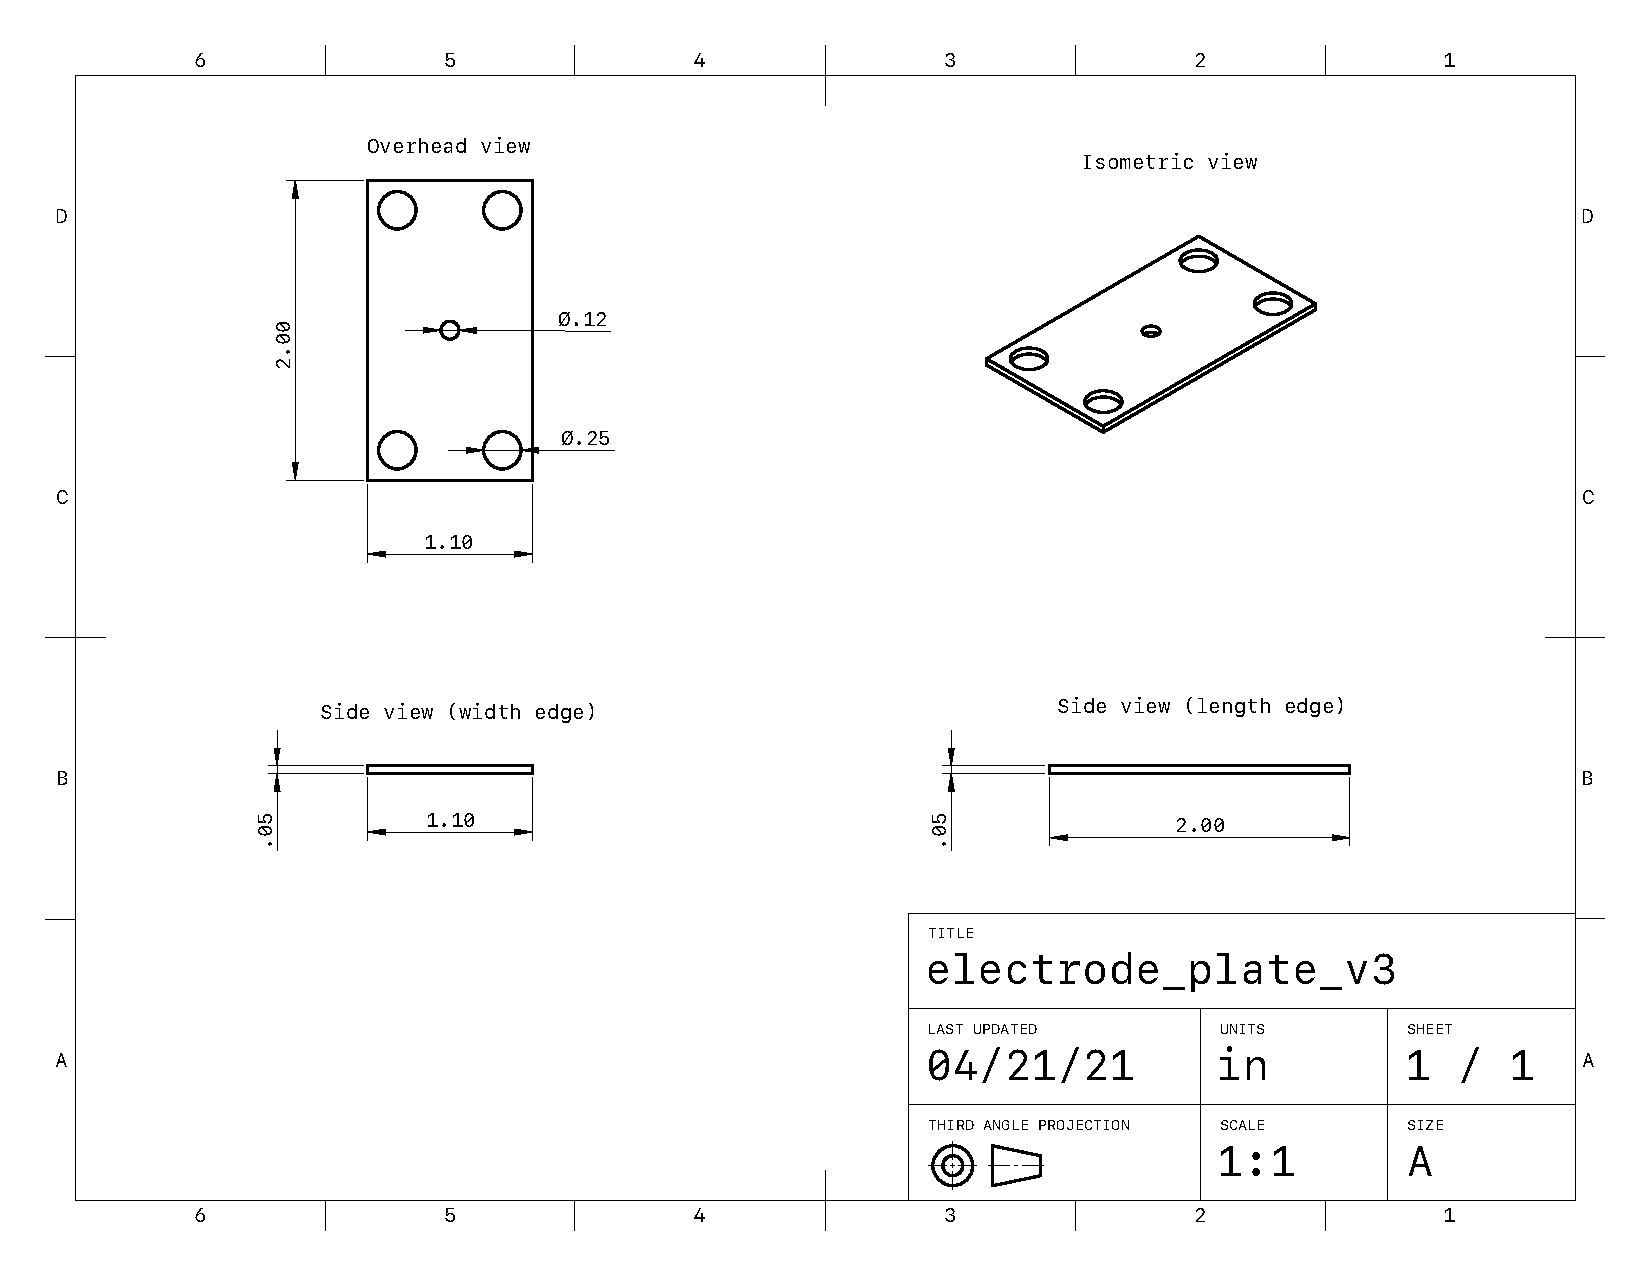
\includegraphics[width=.776\textwidth]{figs/ALGAAS/assemblies/assembly2/assembly2_electrode.pdf}
  \caption{Rectangular (.05"X1.1"X2") plates made of aluminum.}
\end{figure}

\newpage
\subsubsection{Iteration 2.1}
\begin{figure}[!ht]
	\centering
	\begin{subcaptiongroup}
		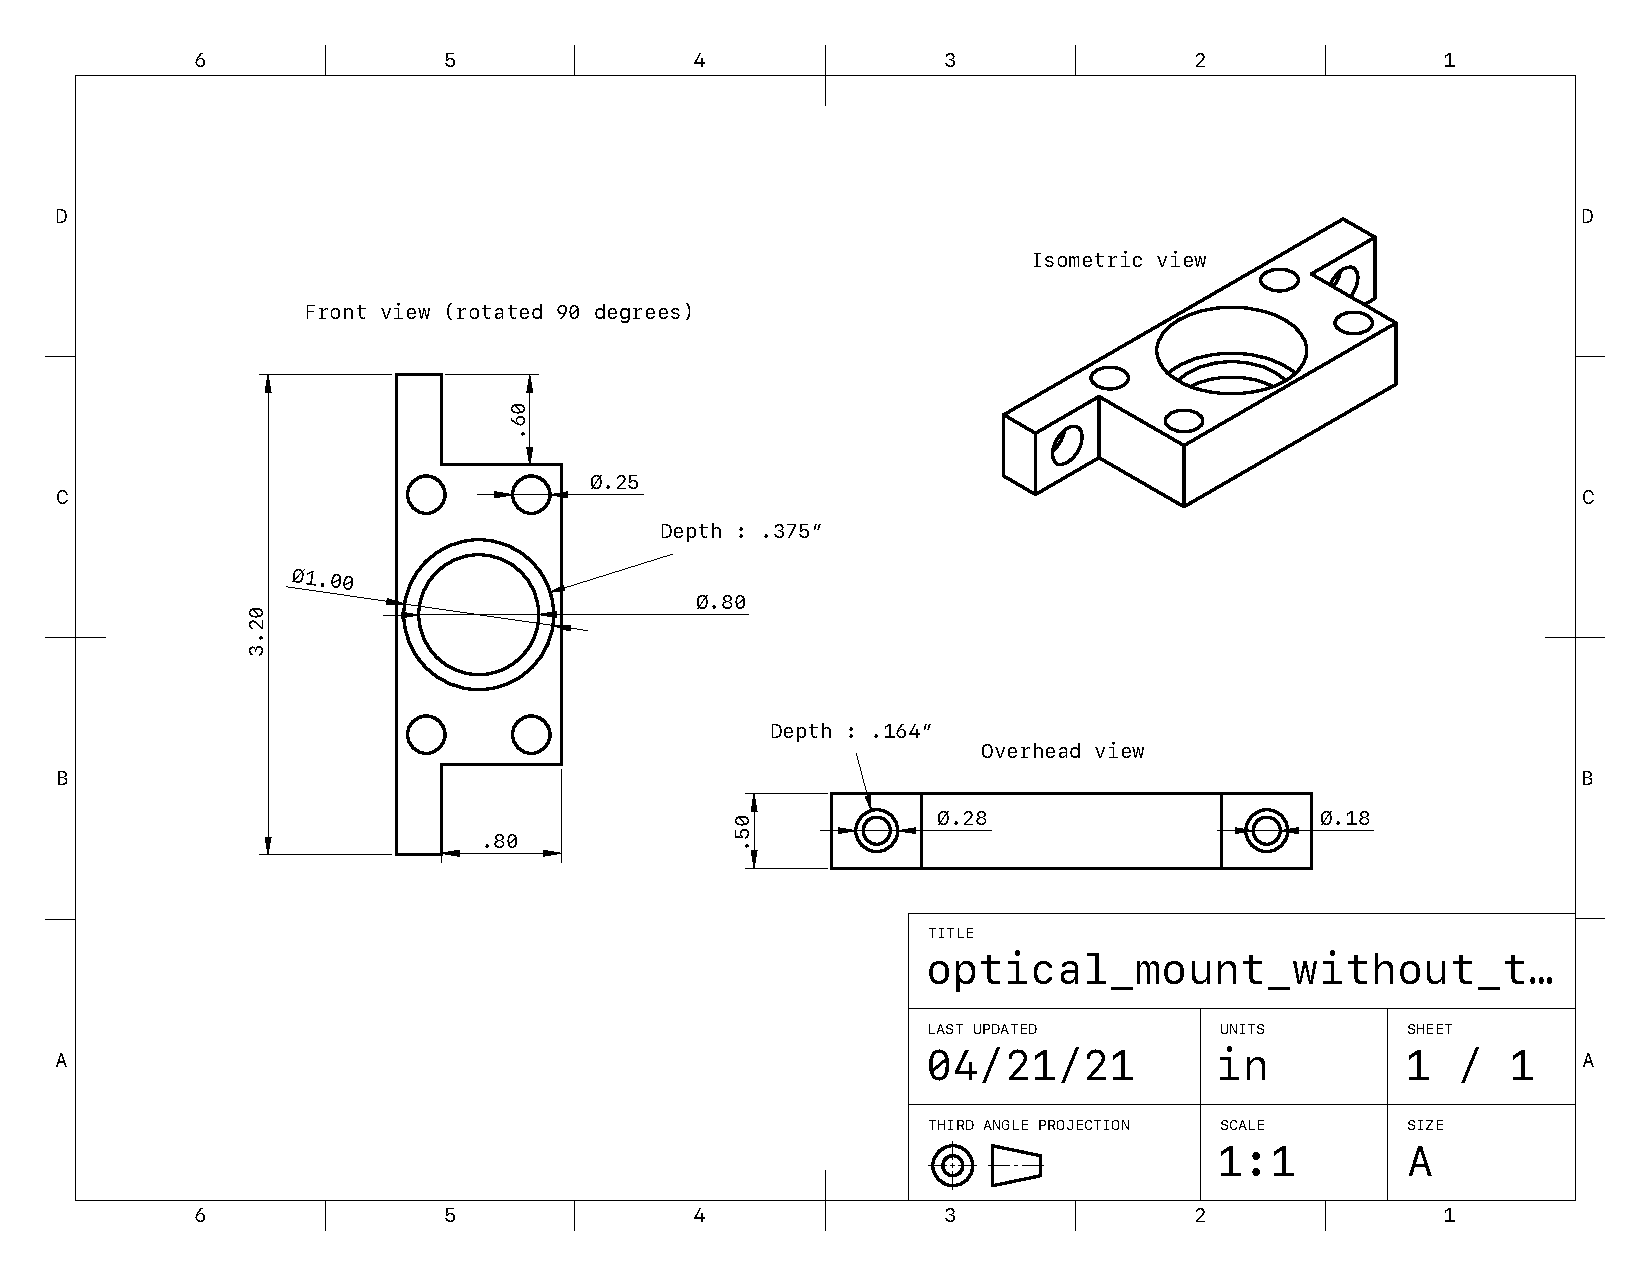
\includegraphics[width=.76\textwidth]{figs/ALGAAS/assemblies/assembly2/assembly2_PVC_mount.pdf}
		\phantomcaption\label{A2PVCmount}
		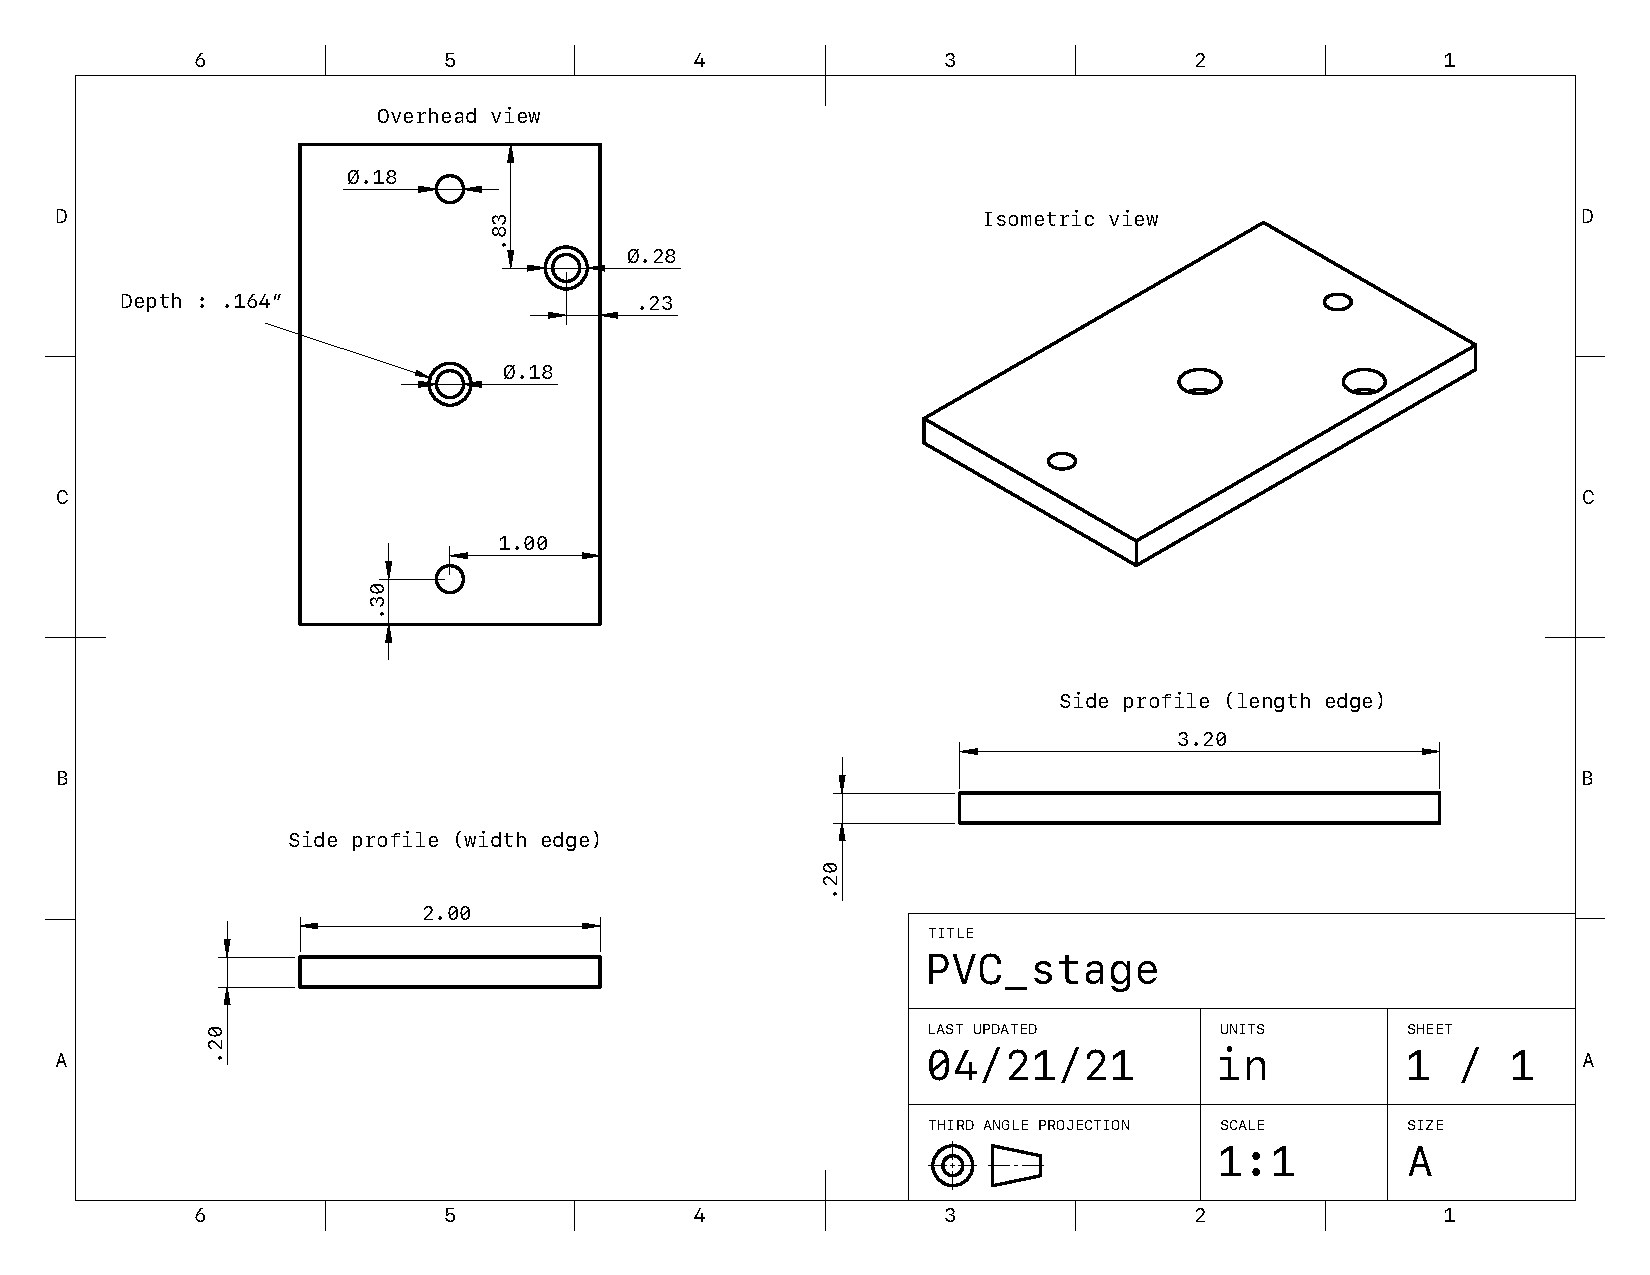
\includegraphics[width=.76\textwidth]{figs/ALGAAS/assemblies/assembly2/assembly2_PVC_stage.pdf}
		\phantomcaption\label{A2PVCstage}
	\end{subcaptiongroup}
	\caption{A design iteration of the assembly 2 mounts. Materials tried varied from PVC, PLA, and PETG. Quarter inch holes are bored in order to pass nylon screws holding electrode plates fixed to the mount.}
	\label{fig:assembly2bp}
\end{figure}
\FloatBarrier

\subsubsection{Iteration 2.2}

\subsubsection{3D printed w/ MACOR spacers}

\textcolor{red}{Insert blueprints}

\textcolor{red}{Insert printed results}

\newpage

\section{Assembly 3 [MACOR] (blueprint)}
\subsubsection{Cross section}
\subsubsection{Electrodes}

\subsubsection{Iteration 3.0}
\begin{figure}[H]
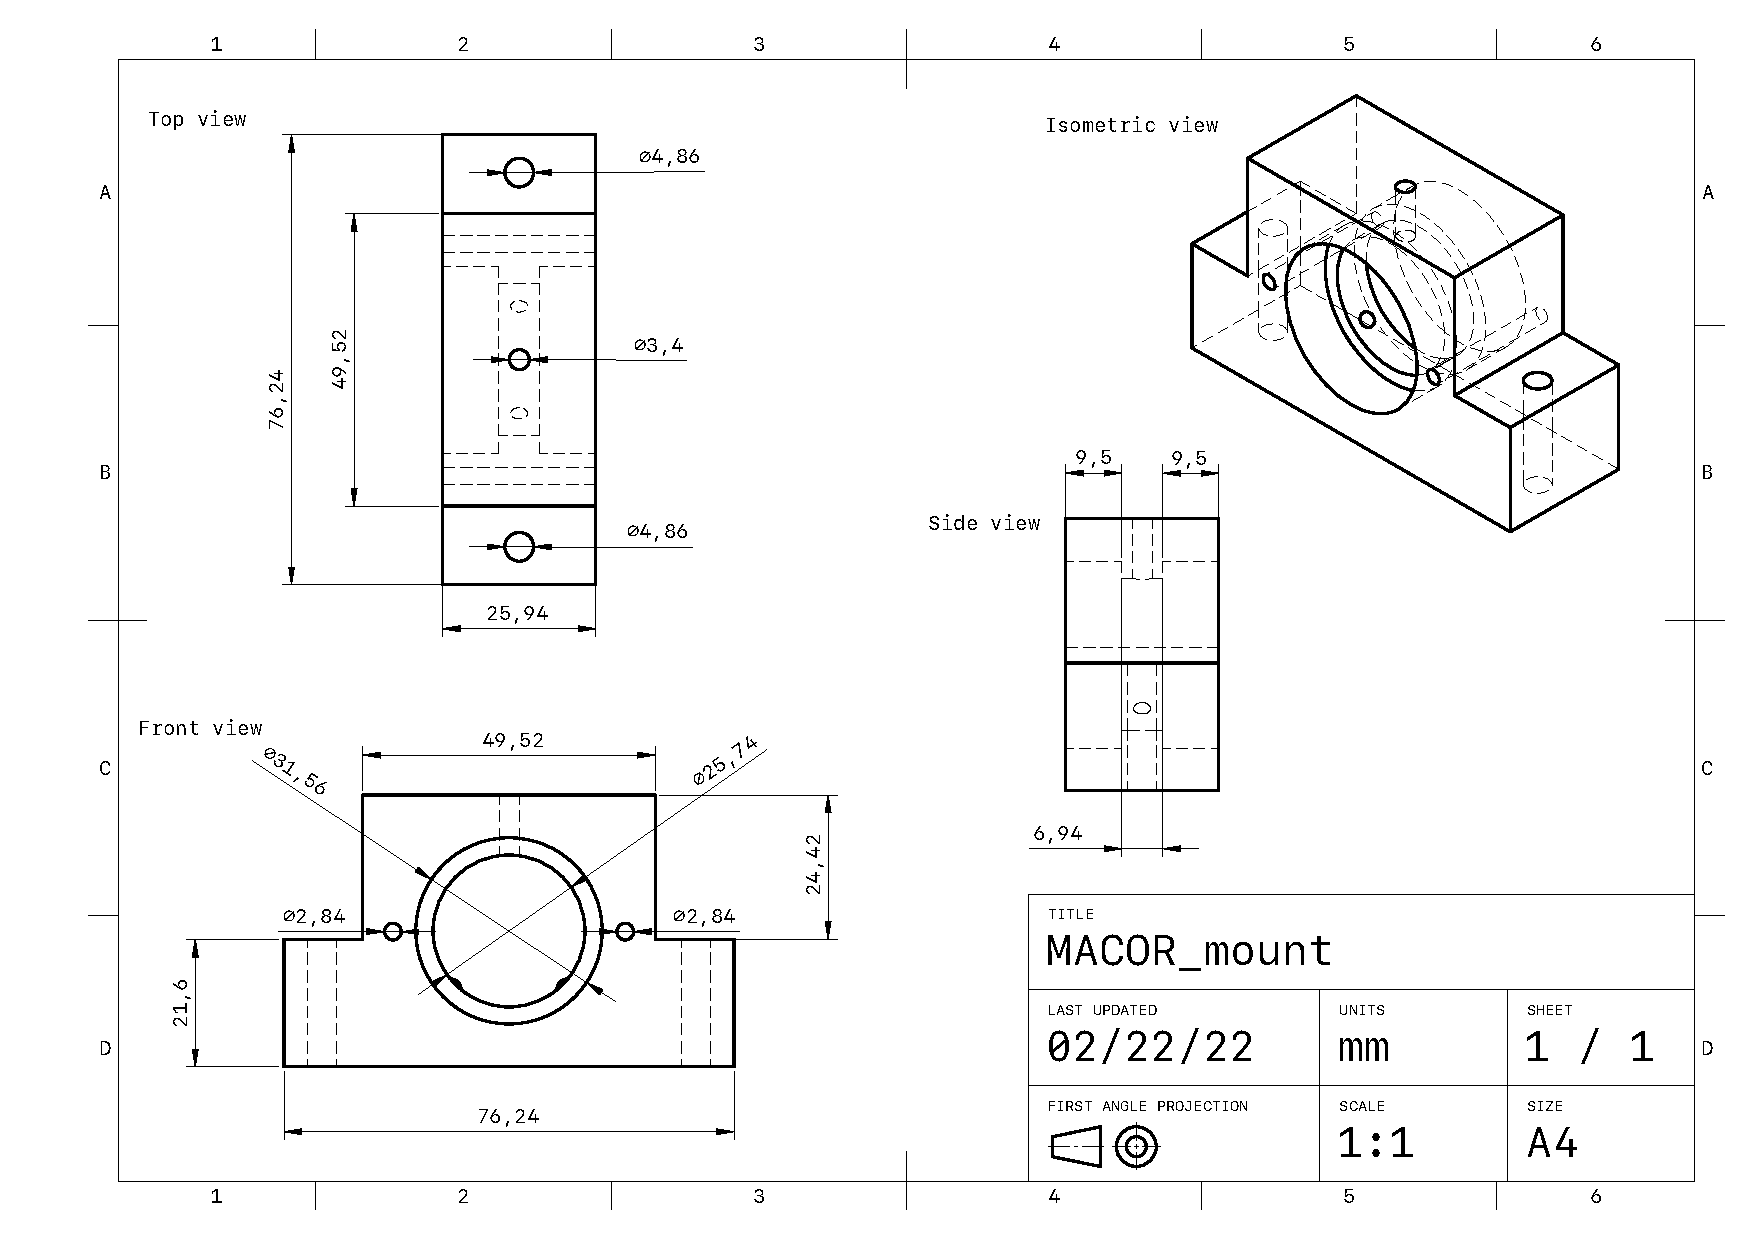
\includegraphics[width=\textwidth]{figs/ALGAAS/assemblies/assembly3/MACOR_mount.pdf}
\caption{MACOR mount design constucted in Shapr3D}
\label{fig:macormountdesign}
\end{figure}

\mbox{}
\vfill

\section{Calibration}\label{sec:calibration}
%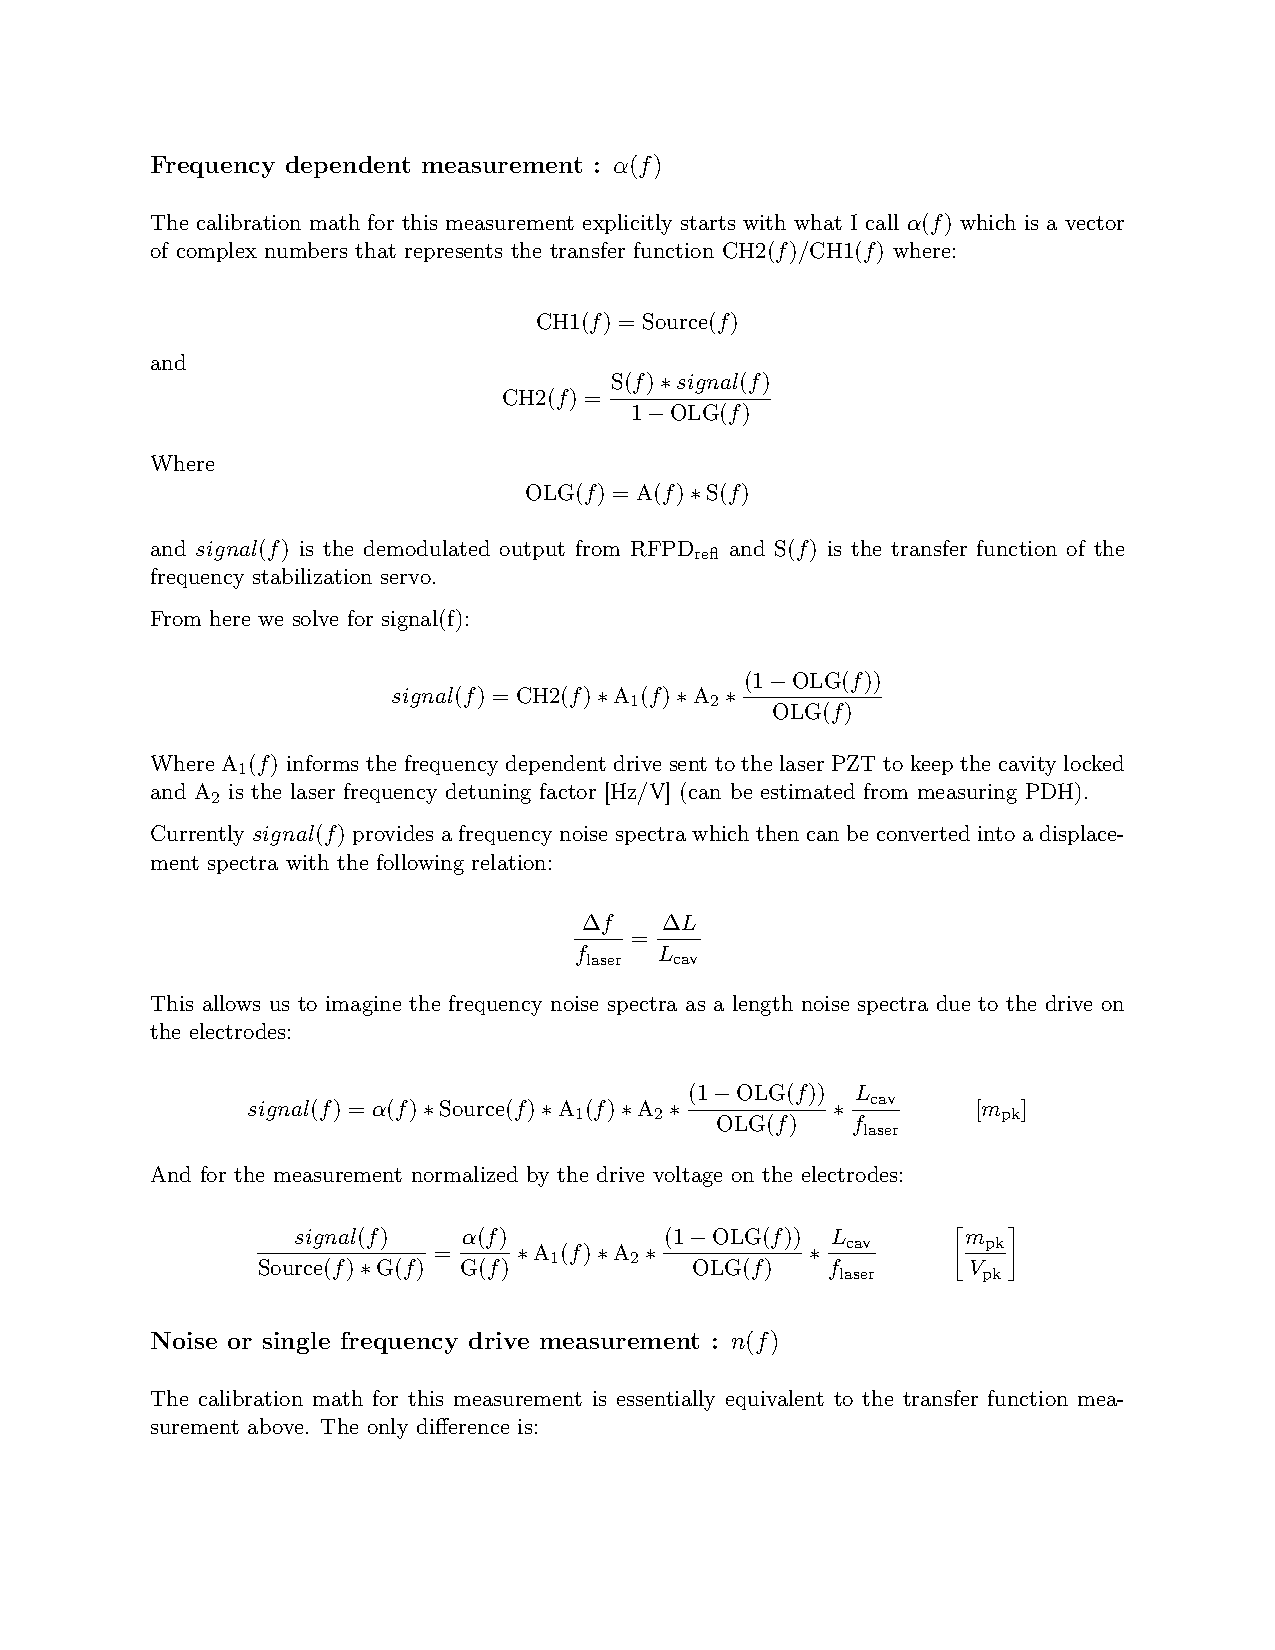
\includepdf[pages=-, pagecommand={}]{notes/pockels_calibration.pdf}
The calibration math for this measurement explicitly starts with what I
call \(\alpha(f)\) which is a vector of complex numbers that represents
the transfer function \(\mathrm{CH2}(f)/\mathrm{CH1}(f)\) where:

\[\mathrm{CH1}(f) = \mathrm{Source}(f)\] and
\[\mathrm{CH2}(f) = \frac{\mathrm{S}(f)* signal(f)}{1-\mathrm{OLG}(f)}\]

Where \[\mathrm{OLG}(f) = \mathrm{A}(f)* \mathrm{S}(f)\]

and \(signal(f)\) is the demodulated output from
\(\mathrm{RFPD}_\mathrm{refl}\) and \(\mathrm{S}(f)\) is the transfer
function of the frequency stabilization servo.

From here we solve for signal(f):

\[signal(f) = \mathrm{CH2}(f) * \mathrm{A}_{1}(f) * \mathrm{A}_2* \frac{(1-\mathrm{OLG}(f))}{\mathrm{OLG}(f)}\]

Where \(\mathrm{A}_{1}(f)\) informs the frequency dependent drive sent
to the laser PZT to keep the cavity locked and \(\mathrm{A}_2\) is the
laser frequency detuning factor {[}Hz/V{]} (can be estimated from
measuring PDH).

Currently \(signal(f)\) provides a frequency noise spectra which then
can be converted into a displacement spectra with the following
relation:

\[\frac{\Delta f}{f_\mathrm{laser}} = \frac{\Delta L}{L_\mathrm{cav}}\]

This allows us to imagine the frequency noise spectra as a length noise
spectra due to the drive on the electrodes:

\[signal(f) = \alpha(f)* \mathrm{Source}(f) * \mathrm{A}_{1}(f) * \mathrm{A}_2* \frac{(1-\mathrm{OLG}(f))}{\mathrm{OLG}(f)} * \frac{L_\mathrm{cav}}{f_\mathrm{laser}}\hspace{35pt} [m_\mathrm{pk}]\]

And for the measurement normalized by the drive voltage on the
electrodes:

\[\frac{signal(f)}{\mathrm{Source}(f) * \mathrm{G}(f)} = \frac{\alpha(f)}{\mathrm{G}(f)} * \mathrm{A}_{1}(f) * \mathrm{A}_2* \frac{(1-\mathrm{OLG}(f))}{\mathrm{OLG}(f)} * \frac{L_\mathrm{cav}}{f_\mathrm{laser}}\hspace{35pt} \bigg[\frac{m_\mathrm{pk}}{V_\mathrm{pk}}\bigg]\]
\#\# Noise or single frequency drive measurement : \(n(f)\) The
calibration math for this measurement is essentially equivalent to the
transfer function measurement above. The only difference is:

\[\mathrm{CH1}(f) = \frac{\mathrm{S}(f)* signal(f)}{1-\mathrm{OLG}(f)}\]

and

\[signal(f) = \mathrm{CH1}(f) * \mathrm{A}_{1}(f) * \mathrm{A}_2* \frac{(1-\mathrm{OLG}(f))}{\mathrm{OLG}(f)} * \frac{L_\mathrm{cav}}{f_\mathrm{laser}}\]

Where \(signal(f)\) in this measurement represents the free running
cavity displacement noise with the exception of a single frequency if it
is not a noise measurement.

If \(\mathrm{CH1}(f)\) is in \(\frac{V_\mathrm{rms}}{\sqrt{Hz}}\) then
signal(f) will be in \(\frac{m_\mathrm{rms}}{\sqrt{Hz}}\)

or

If \(\mathrm{CH1}(f)\) is in \(V_\mathrm{pk}\) then signal(f) will be in
\(m_\mathrm{pk}\) \#\# Calibration code

\subsubsection{Import packages}\label{import-packages}

If it fails the first time try installing the following to a separate
conda enviornment: {/pydependencies/eo\_calibrate.yml}

\begin{lstlisting}[frame=single, language=Python]
import glob
import numpy as np
import matplotlib.pyplot as plt
from matplotlib import rc
import os
import h5py

plt_style_dir = 'pydependencies/stylelib/'

if os.path.isdir(plt_style_dir) == True:
    plt.style.use(plt_style_dir + 'pptsize')  # This just sets a python figure style (you can adjust it to your preferences)
\end{lstlisting}

\subsubsection{Frequently used
functions:}\label{frequently-used-functions}

\begin{lstlisting}[frame=single, language=Python]
def concat_vecs(directory):
    """
    Takes a directory filled with spectra measurements (from SR785) to be
    concatenated to a single vector. The output of the function is (frequency
    vector, amplitude vector)
    """
    txtcounter = len(glob.glob1(directory,"*.TXT"))
    freq = np.zeros((801,txtcounter))
    freq1 = np.zeros((801,txtcounter))
    vpk = np.zeros((801,txtcounter))

    columns = range(0,txtcounter)
    fff = 0
    vpkn = 0
    ##  import and measurements
    for i in columns:
        data = np.loadtxt(directory + str(i).zfill(2) + '.TXT')
        freq[:,i] = data[:,0]
        vpk[:,i] = data[:,1]
        if i == columns[0]:
            fff = freq[:,i]
            vpkn = vpk[:,i]
        elif i == columns[-1]:
            fff = np.append(fff,freq[:,i])
            vpkn=np.append(vpkn,vpk[:,i])
        else:
            fff = np.append(fff, freq[:,i][:-1])
            vpkn = np.append(vpkn, vpk[:,i][:-1])
    return fff, vpkn

def gen_concat_vecs(directory):
    """
    Takes a directory filled with spectra measurements (from SR785) to be
    concatenated to a single vector. The output of the function is (frequency
    vector, amplitude vector)
    """
    txtcounter = len(glob.glob1(directory,"*.TXT"))
    columns = range(0,txtcounter)

    data = np.loadtxt(directory + str(0).zfill(2) + '.TXT')
    master_freq = data[:,0]
    master_data = data[:,1]

    for i in columns:
        if i < columns[-1]:
            data = np.loadtxt(directory + str(i).zfill(2) + '.TXT')
            data1 = np.loadtxt(directory + str(i+1).zfill(2) + '.TXT')
            xy, xind, yind = np.intersect1d(data[:,0], data1[:,0], \
            return_indices=True)

            if sum(yind>400) != 0:
                xy2, xind2, yind2 = np.intersect1d(master_freq, data1[390:,0],\
                return_indices=True)
                master_freq = np.append(master_freq[:(xind2[0]-11)], \
                data1[390:,0])
                master_data = np.append(master_data[:(xind2[0]-11)], \
                data1[390:,1])

            else:
                if len(xy) != 0:
                    master_freq = np.append(master_freq, data1[yind[-1]+1:,0])
                    master_data = np.append(master_data, data1[yind[-1]+1:,1])
                else:
                    master_freq = np.append(master_freq, data1[:,0])
                    master_data = np.append(master_data, data1[:,1])

    return master_freq, master_data

def transfer_function(amplitude, phase):
    """
    Takes frequency response data (amplitude and phase) combines it into a
    transfer function : Ae^(i*phi)
    """
    return 10**(amplitude/20)* np.exp(1j*(phase/180)*np.pi)

def phase_wrap(phase_array, type='deg'):
    """
    Wraps phase from -180 -> +180 degrees if type == 'rad' then it wraps from
    -pi -> pi
    """
    if type == 'deg':
        fin_phase_array = (phase_array + 180) % (2 * 180) - 180
    if type == 'rad':
        fin_phase_array = (phase_array + np.pi) % (2 * np.pi) - np.pi
    return fin_phase_array

def function_transfer(freq,tf_in):
    """
    Converts transfer function back to amplitude and phase data (frequency, amplitude [dB], phase [deg])
    """
    db = 20*np.log10(abs(tf_in))
    deg = np.angle(tf_in, deg=True)
    return freq, db, deg

def tf_import(tf_path):
    """
    Takes a directory containing amplitude and phase data (dB and deg) and
    imports the data and outputs (frequency, amplitude, phase)
    """
    db = np.loadtxt(tf_path + 'db.TXT')
    deg = np.loadtxt(tf_path + 'deg.TXT')
    ff = db[:,0]
    return ff, db[:,1], deg[:,1]

def tf_interpolate(new_freq, tf_tuple):
    """

    """
    new_db = np.interp(new_freq, tf_tuple[0], tf_tuple[1])
    new_deg = np.interp(new_freq, tf_tuple[0], tf_tuple[2])
    return new_freq, new_db, new_deg

def bode_plt(tf_tuple, save_path, lbl, title, ylbl='dB'):
    ff = tf_tuple[0]
    db = tf_tuple[1]
    deg = tf_tuple[2]
    bode_fig = plt.figure()
    plt.subplot(211)
    if not ylbl=='dB':
        plt.loglog(ff, db, label=lbl)
    else:
        plt.semilogx(ff,db, label = lbl)
    plt.xlim(ff[0], ff[-1])
    plt.ylabel(ylbl)
    plt.legend()
    plt.title(title.replace('_', '\_'))
    plt.subplot(212)
    plt.semilogx(ff,deg, label = lbl)
    plt.xlim(ff[0], ff[-1])
    plt.legend()
    plt.xlabel('Frequency [Hz]')
    plt.ylabel('phase [deg]')
    plt.savefig(save_path + '/' + title + '.png', dpi=300,bbox_inches='tight')
    plt.close()
    return bode_fig

def h5_import(dir):
    return h5py.File(dir + '/data.hdf5', 'r')

def printname(name):
    print(name)

def h5_peek(h5_file):
    if type(h5_file) == str:
        h5_data = h5_import(h5_file)
    else:
        h5_data = h5_file

    return h5_data.visit(printname)

def qkh5plt(h5_file,meas,lbl,axis,yax='log',lgnd_size=30,peek=False):
    """
    Plotting tool that allows you to quickly plot any one of the traces from an
    h5 file.

    h5_file : Can be an already open h5 file or a directory to an h5 file

    meas : The measurement you wish to select from the options in the h5 file

    axis : needs to inherit axis from already established figure

    lbl : Label we want to tag onto the requested dataset

    yax : can swap between a logrithmic and linear yaxis

    lgnd_size : size of legend font
    """

    if type(h5_file) == str:
        h5_data = h5_import(h5_file)
    else:
        h5_data = h5_file

    if peek == True:
        h5_peek(h5_file)

    if yax == 'log':
        axis.loglog(h5_data['freq'][:],h5_data[meas][:],label=lbl)
    elif yax == 'lin':
        axis.semilogx(h5_data['freq'][:],h5_data[meas][:],label=lbl)

    axis.legend(prop={'size':lgnd_size})
    plt.xlim(h5_data['freq'][0],h5_data['freq'][-1])

\end{lstlisting}

\subsubsection{Input variables}\label{input-variables}

\begin{lstlisting}[frame=single, language=Python]
meas_data_dir = 'measurements/swept/algaas/08_13_2021/meas1/'                                # directory where the uncalibrated data lives
date = '08_13_2021'                                                              # date when measurement was taken ("mm_dd_yyyy")
final_dir = 'results/'                                                           # directory where the final data will live
meas_type = 'swept'                                                              # type of measurement taken tag (i.e. noise, swept)
spectra_type = 'pk'                                                              # spectra type (i.e. pk, rms)
sample = 'algaas'                                                                # sample tag (i.e. algaas, atfilms, sio2tao5, etc.)
xtradir = 'meas1'                                                                # this label helps distinguish between measurements taken in a given day
cav_length = .165                                                                # recorded length of cavity
inp_voltage_swept = 4.65                                                         # voltage sent from SR785 to HVA connected to electrodes
plot_saving = False                                                              # generate and save .png files for intermediate calibration functions
model = False                                                                    # boolean that decides whether or not the model estimate should be plotted with calibrated data
\end{lstlisting}

\begin{lstlisting}[frame=single, language=Python]
labl = date + '_' + meas_type + '_'  + spectra_type + '_' + sample               # label of the directory containing all the figures and .h5 file
if xtradir != 'none':                                                            # adjusted label if an extra directory was used
    labl = date + '_' + meas_type + '_' + spectra_type + '_' + xtradir +  \
    '_' + sample
new_final_dir = final_dir + '/' + labl


if os.path.isdir(new_final_dir) == False:                                        # generates the directory containing the results if it doesn't already exist
    os.mkdir(new_final_dir)
\end{lstlisting}

\subsubsection{Data import}\label{data-import}

\begin{lstlisting}[frame=single, language=Python]
#HVA and OLG directory search
HVA_common_dir = 'measurements/HVASVR_tf/'                             # HVA and OLG directories
OLG_common_dir = 'measurements/OLG/'
HVA_dir = HVA_common_dir + 'HVACH3_plus_pomona/' + date + '/'
#OLG_dir = OLG_common_dir + date + '/'
OLG_dir = OLG_common_dir + sample + '/' + date + '/'


if xtradir != 'none' and meas_type != 'noise':
    HVA_dir = HVA_dir + xtradir + '/'
    OLG_dir = OLG_dir + xtradir + '/'

HVA = tf_import(HVA_dir)                                                     # import the HVA and OLG data
OLG = tf_import(OLG_dir)
#If the data is a swept frequency measurement
if meas_type == 'swept':                                                     # import HVA CH1 transfer function data for transfer function measurement
    HVA_CH1_dir = HVA_common_dir + 'HVACH1/' + date + '/'
    #HVA_CH1_dir = HVA_common_dir + 'HVACH1_w_LPF/' + date + '/'
    if xtradir != 'none':
        HVA_CH1_dir = HVA_CH1_dir + xtradir + '/'

    electrode_type = 'disk'                                                  # import low pass measurement from resistor / electrode capacitence
    if sample == 'sio2ta2o5' or sample == 'atfilms':
        Electcap_dir = 'measurements/electrode_capacitence/' + \
        electrode_type + '/' + sample + '/03_29_2021/'
    if sample == 'atfilms':
        Electcap_dir = 'measurements/electrode_capacitence/' + \
        electrode_type + '/' + sample + '/06_04_2021/'
    if sample == 'algaas':
        Electcap_dir = 'measurements/electrode_capacitence/' + \
        electrode_type + '/' + sample + '/03_10_2021/'

    meas_swep = tf_import(meas_data_dir)                                     # import transfer function measurement
    if plot_saving == True:                                                  # plot uncalibrated transfer function measurement if requested
        bode_plt(meas_swep, new_final_dir, date.replace("_", "\_"), \
        'Pockels_effect_frequency_response_uncalibrated_dB')

    swept_tf = transfer_function(meas_swep[1], meas_swep[2])                 # combine amplitude and phase

    HVA_CH1 = tf_import(HVA_CH1_dir)                                         # HVA CH1 import and interpolation (interpolate to transfer function frequency vector)
    HVA_CH1_inter = tf_interpolate(meas_swep[0], HVA_CH1)
    HVA_CH1_tf = transfer_function(HVA_CH1_inter[1], HVA_CH1_inter[2])

    #Electrode capacitence transfer function import and interpolation
    ECAP = tf_import(Electcap_dir)                                           # Import and interpolate LPF measurement (part of frequency dependent drive to electrodes)
    ECAP_inter = tf_interpolate(meas_swep[0], ECAP)
    ECAP_tf = transfer_function(ECAP_inter[1], ECAP_inter[2])

    #interpolate related tfs
    HVA_inter = tf_interpolate(meas_swep[0], HVA)                            # HVA CH3 and OLG interpolation
    OLG_inter = tf_interpolate(meas_swep[0], OLG)

else:                                                                        # if the measurement is not a transfer function (spectra measurement)
    spectra = gen_concat_vecs(meas_data_dir)                                 # changed from concat_vecs to gen_concat_vecs (07-25-2021)
    #interpolate related tfs
    HVA_inter = tf_interpolate(spectra[0], HVA)                              # HVA CH3 and OLG interpolation
    OLG_inter = tf_interpolate(spectra[0], OLG)
    if plot_saving == True:
        #Spectra plotting
        plt.loglog(spectra[0], spectra[1], label=labl.replace("_","\_"))
        plt.legend()
        plt.xlabel('frequency [Hz]')
        #plt.xlim([spectra[0][0],spectra[0][-1]])
        if spectra_type == 'pk':
            plt.ylabel('$$V_\mathrm{pk}$$')
        elif spectra_type == 'rms':
            plt.ylabel('$$V_\mathrm{rms}$$')
        plt.savefig(new_final_dir + '/v_spectra_' + labl + '.png',dpi=300, \
        bbox_inches='tight')
        plt.close()
        
        
if plot_saving == True:                                                      # plot and HVACH3 and OLG if requested
    #HVA plotting
    bode_plt(HVA, new_final_dir, 'HVA.75\_total\_gain', 'HVACH3+pomona')
    #OLG plotting
    bode_plt(OLG, new_final_dir , date.replace('_', '\_'), 'OLG' )
\end{lstlisting}

\subsubsection{Build calibration
function}\label{build-calibration-function}

\begin{lstlisting}[frame=single, language=Python]
HVA_tf = transfer_function(HVA_inter[1], HVA_inter[2])                       # combine amplitude and phase of HVACH3 and OLG
OLG_tf = transfer_function(OLG_inter[1], OLG_inter[2])

if meas_type == 'swept':
    volt_divider = False                                                     # Voltage divider if you want a smaller normalization factor
    if volt_divider == True:                                                 # Voltage divider with r_1 as the first resistor and r_2 as the resistor connected to ground
        r_1 = 100000
        r_2 = 50
        pom_vdivider = (r_2)/(r_1+r_2)

        swept_tf = swept_tf*pom_vdivider
    else:
        pom_vdivider = 1

    stf_unnorm = swept_tf*inp_voltage_swept                                  # Unnormalized transfer function measurement

    s_unnorm = [meas_swep[0], abs(stf_unnorm), np.angle(stf_unnorm,  \
    deg=True)]                                                               # Unnormalized transfer function in triad format

    if plot_saving == True:                                                  # Plot voltage spectra for transfer function measurement if requested
        bode_plt(s_unnorm, new_final_dir, date.replace('_','\_'), \
        'Pockels_effect_frequency_response_vspectra', \
        ylbl='$V_\mathrm{pk}$')

    v_direct = inp_voltage_swept*HVA_CH1_tf*ECAP_tf                          # This is the voltage directly across the coating for all measured frequencies (with phase information)
    vdirec = [meas_swep[0], abs(v_direct), np.angle(v_direct,deg=True)]      # Frequency dependent injection voltage (transfer function triad)
    if plot_saving==True:                                                    # Plot frequency dependent injection voltage if requested
        bode_plt(vdirec, new_final_dir, date.replace('_','\_'), \
        'Potential difference across electrodes', ylbl='$V_\mathrm{pk}$')


#laserV2Hz = 2.0e6
#laserV2Hz = 1.4706e6                                                        # measurement from elog 831 (05-24-2021)
laserV2Hz = 1.748e6                                                          # Laser PZT response acquired from PDH measurement
HzpV = HVA_tf*laserV2Hz                                                      # Actuation function A(f) = A_1(f)*A_2(f)

CLG = 1/(1-OLG_tf)                                                           # Closed loop gain
CAL = OLG_tf*CLG                                                             # Loop gain calibration factor
#CALVpHz=CAL/HzpV                                                            # Calibrated voltage to frequency
CALHzpV=HzpV/CAL                                                             # Calibration factor using A(f) and OLG(f)

if meas_type == 'swept':                                                     # Calibrate data
    freq_noise = CALHzpV*stf_unnorm
else:
    freq_noise = abs(CALHzpV)*spectra[1]

if plot_saving == True and meas_type != 'swept':                             # if plotting spectra measurement this is plotting and saving the frequency noise if requested
    plt.loglog(spectra[0],freq_noise, label= date.replace('_', '\_'), \
    linewidth=3)
    #plt.xlim([spectra[0][0], spectra[0][-1]])
    plt.legend()
    plt.xlabel('Frequency [Hz]')
    plt.ylabel('$$\mathrm{Hz}_\mathrm{pk}$$')
    plt.title("Laser frequency noise from measured voltage noise")
    plt.savefig(new_final_dir + '/Hz' + '_spectra_' + labl + '.png', \
    dpi=300, bbox_inches='tight')
    plt.close()
\end{lstlisting}

\subsubsection{Cavity params}\label{cavity-params}

\begin{lstlisting}[frame=single, language=Python]
c = 299792458                                                                # Cavity parameters
lamb =1.064e-6
nu = c/lamb
Lcav = cav_length
\end{lstlisting}

\subsubsection{Calibrate voltage to
displacement}\label{calibrate-voltage-to-displacement}

\begin{lstlisting}[frame=single, language=Python]
#Displacement spect
displac_spect = freq_noise*Lcav/nu                                           # Calibrate to displacement spectra
if meas_type == 'swept':
    disp_spect_norm = displac_spect/v_direct                                 # Displacement spectra normalized by the frequency dependent injection (leaves us with mpk/Vpk)

model_freq = 10000                                                           # Model estimate
marty_estimate = 3.8e-16                                                     # mpk/[V*m]
Efield_strength_estimate = 4648                                              # [V/m] (changed from 6350 to 4648 on 07-13-2021)

#Displacement spectra
if  meas_type == 'swept':                                                    # Organizing and plotting displacement spectra
    displac_spect_unnorm = [meas_swep[0], abs(displac_spect), \
    np.angle(displac_spect, deg=True)]
    displac_spect_norm = [meas_swep[0], abs(disp_spect_norm), \
    np.angle(disp_spect_norm, deg=True)]
    final_fig = bode_plt(displac_spect_unnorm, new_final_dir, \
    date.replace('_','\_'), \
    'Displacement spectra for AlGaAs Pockels effect measurement', \
    ylbl='Displacement [$\mathrm{m}_\mathrm{pk}$]')
else:
    final_fig = plt.loglog(spectra[0],abs(displac_spect),color='m', \
    label=labl, linewidth=3)
    plt.xlabel('frequency [Hz]')
    #plt.xlim([spectra[0][0], spectra[0][-1]])
    #plt.ylabel('$V_\mathrm{{}}$'.format(spectra_type))

if model == True and meas_type != 'swept':                                   # If model estimate is requested, will plot model estimate with data
    plt.axhline(y=marty_estimate*Efield_strength_estimate,linestyle='--', \
    color='k', label='Marty estimate')
    #plt.xlim([spectra[0][0], spectra[0][-1]])
    plt.legend()
    plt.xlabel('Frequency [Hz]')
    if spectra_type == 'pk':
        plt.ylabel('Displacement [$\mathrm{m}_\mathrm{pk}$]')
    if spectra_type == 'rms':
        plt.ylabel('Displacement [$\mathrm{m}_\mathrm{rms}$]')
    plt.title("Displacement spectra for AlGaAs Pockels effect measurement")
    plt.savefig(new_final_dir + '/' + 'pockels_displacement_spectra' + \
    labl + '.png',dpi=300,bbox_inches='tight')
\end{lstlisting}

\subsubsection{Save raw data, calibration functions, calibrated
displacement function, and other
metadata}\label{save-raw-data-calibration-functions-calibrated-displacement-function-and-other-metadata}

\begin{lstlisting}[frame=single, language=Python]
with h5py.File(new_final_dir + "/data.hdf5", "a") as f:                      # Store raw / calibrated data along with metadata in data directory

    #Raw data
    raw = f.create_group("raw")
    hva_save = f.create_group("raw/hva")                                     # where hva data will be saved
    hva_save_ch3 = f.create_group("raw/hva/ch3+pomona")
    if meas_type == 'swept':
        freq = f.create_dataset("freq", data=meas_swep[0])                   # common frequency vector
        hva_save_ch1 = f.create_group("raw/hva/ch1")
        hva_save_ch1.attrs['dir'] = HVA_CH1_dir
        pomona_vdiv=f.create_dataset("pomona_vdivider",data=pom_vdivider)    # Voltage divider factor
        trans_func = f.create_group("raw/meas_freq_resp")
        meas_db = f.create_dataset("raw/meas_freq_resp/db", \
        data=meas_swep[1])
        meas_deg = f.create_dataset("raw/meas_freq_resp/deg", \
        data=meas_swep[2])
        trans_func.attrs['dir'] = meas_data_dir
        direc_volt = f.create_group("raw/vdirect")                           # the Vpk voltage and phase information of the signal directly sent to the electrodes
    else:
        freq = f.create_dataset("freq", data=spectra[0])                     # common frequency vector
        vdata_save = f.create_dataset("raw/v_spect", data=spectra[1])
        vdata_save.attrs['units'] = spectra_type
        vdata_save.attrs['dir'] = meas_data_dir                              # where error signal spectra will be saved
    cav_length = f.create_dataset("cav_length", data=Lcav)
    laser_freq = f.create_dataset("laser_freq", data=nu)
    laserPZTresp = f.create_dataset("laserV2Hz", data=laserV2Hz )
    hva_save_ch3.attrs['dir'] = HVA_dir
    olg_save = f.create_group("raw/olg")                                     # where olg data will be saved
    cal_save = f.create_group("raw/cal")                                     # easily accessible loop calibration factor data
    olg_save.attrs['dir'] = OLG_dir
    if meas_type == 'swept':
        hvadb_save_ch1 = f.create_dataset("raw/hva/ch1/db",data=HVA_CH1[1])
        hvadeg_save_ch1 = f.create_dataset("raw/hva/ch1/deg", \
        data=HVA_CH1[2])
        vdirec_db = f.create_dataset("raw/vdirect/db", data=vdirec[1])
        vdirec_deg = f.create_dataset("raw/vdirect/deg", data=vdirec[2])
    hvadb_save_ch3 = f.create_dataset("raw/hva/ch3+pomona/db", \
    data=HVA_inter[1])
    hvadeg_save_ch3 = f.create_dataset("raw/hva/ch3+pomona/deg", \
    data=HVA_inter[2])
    olgdb_save = f.create_dataset("raw/olg/db", data=OLG_inter[1])
    olgdeg_save = f.create_dataset("raw/olg/deg", data=OLG_inter[2])
    calgain_save = f.create_dataset("raw/cal/gain", data=abs(CAL))
    caldeg_save = f.create_dataset("raw/cal/deg", data=np.angle(CAL, \
    deg=True))


    #Calibrated data
    calibra = f.create_group("calibrated")
    hvatf_save = f.create_group("calibrated/hva")
    hvach3tf_save = f.create_dataset("calibrated/hva/ch3+pomona",\
    data=HVA_tf)
    olgtf_save = f.create_dataset("calibrated/olg",data=OLG_tf)
    freqnoise_save = f.create_dataset("calibrated/HzpV",data=CALHzpV)
    if meas_type == 'swept':
        hvach1tf_save = f.create_dataset("calibrated/hva/ch1",\
        data=HVA_CH1_tf)
        displacement_spect = f.create_dataset("calibrated/disp_spect_unnorm"\
        , data=displac_spect_unnorm[1])
        phase_resp1 = f.create_dataset("calibrated/phase_resp_unnorm", \
        data=displac_spect_unnorm[2])
        displacement_spect_norm = \
        f.create_dataset("calibrated/disp_spect_norm", \
        data=displac_spect_norm[1])
        displacement_spect_norm.attrs['units'] = 'm' + spectra_type + '/Vpk'
        phase_resp2 = f.create_dataset("calibrated/phase_resp_norm", \
        data=displac_spect_norm[2])

    else:
        displacement_spect = f.create_dataset("calibrated/disp_spect",\
        data=displac_spect)
    displacement_spect.attrs['units'] = spectra_type
    displacement_spect.attrs['meas_type'] = meas_type
    f.close()
\end{lstlisting}


\section{Single frequency}

\section{Laplace calculator / code}

\textcolor{red}{Snippets of explicit code with a block diagram for clarity}

\section{HVA}

\section{FSS}

\begin{figure}[H]
  \begin{center}
    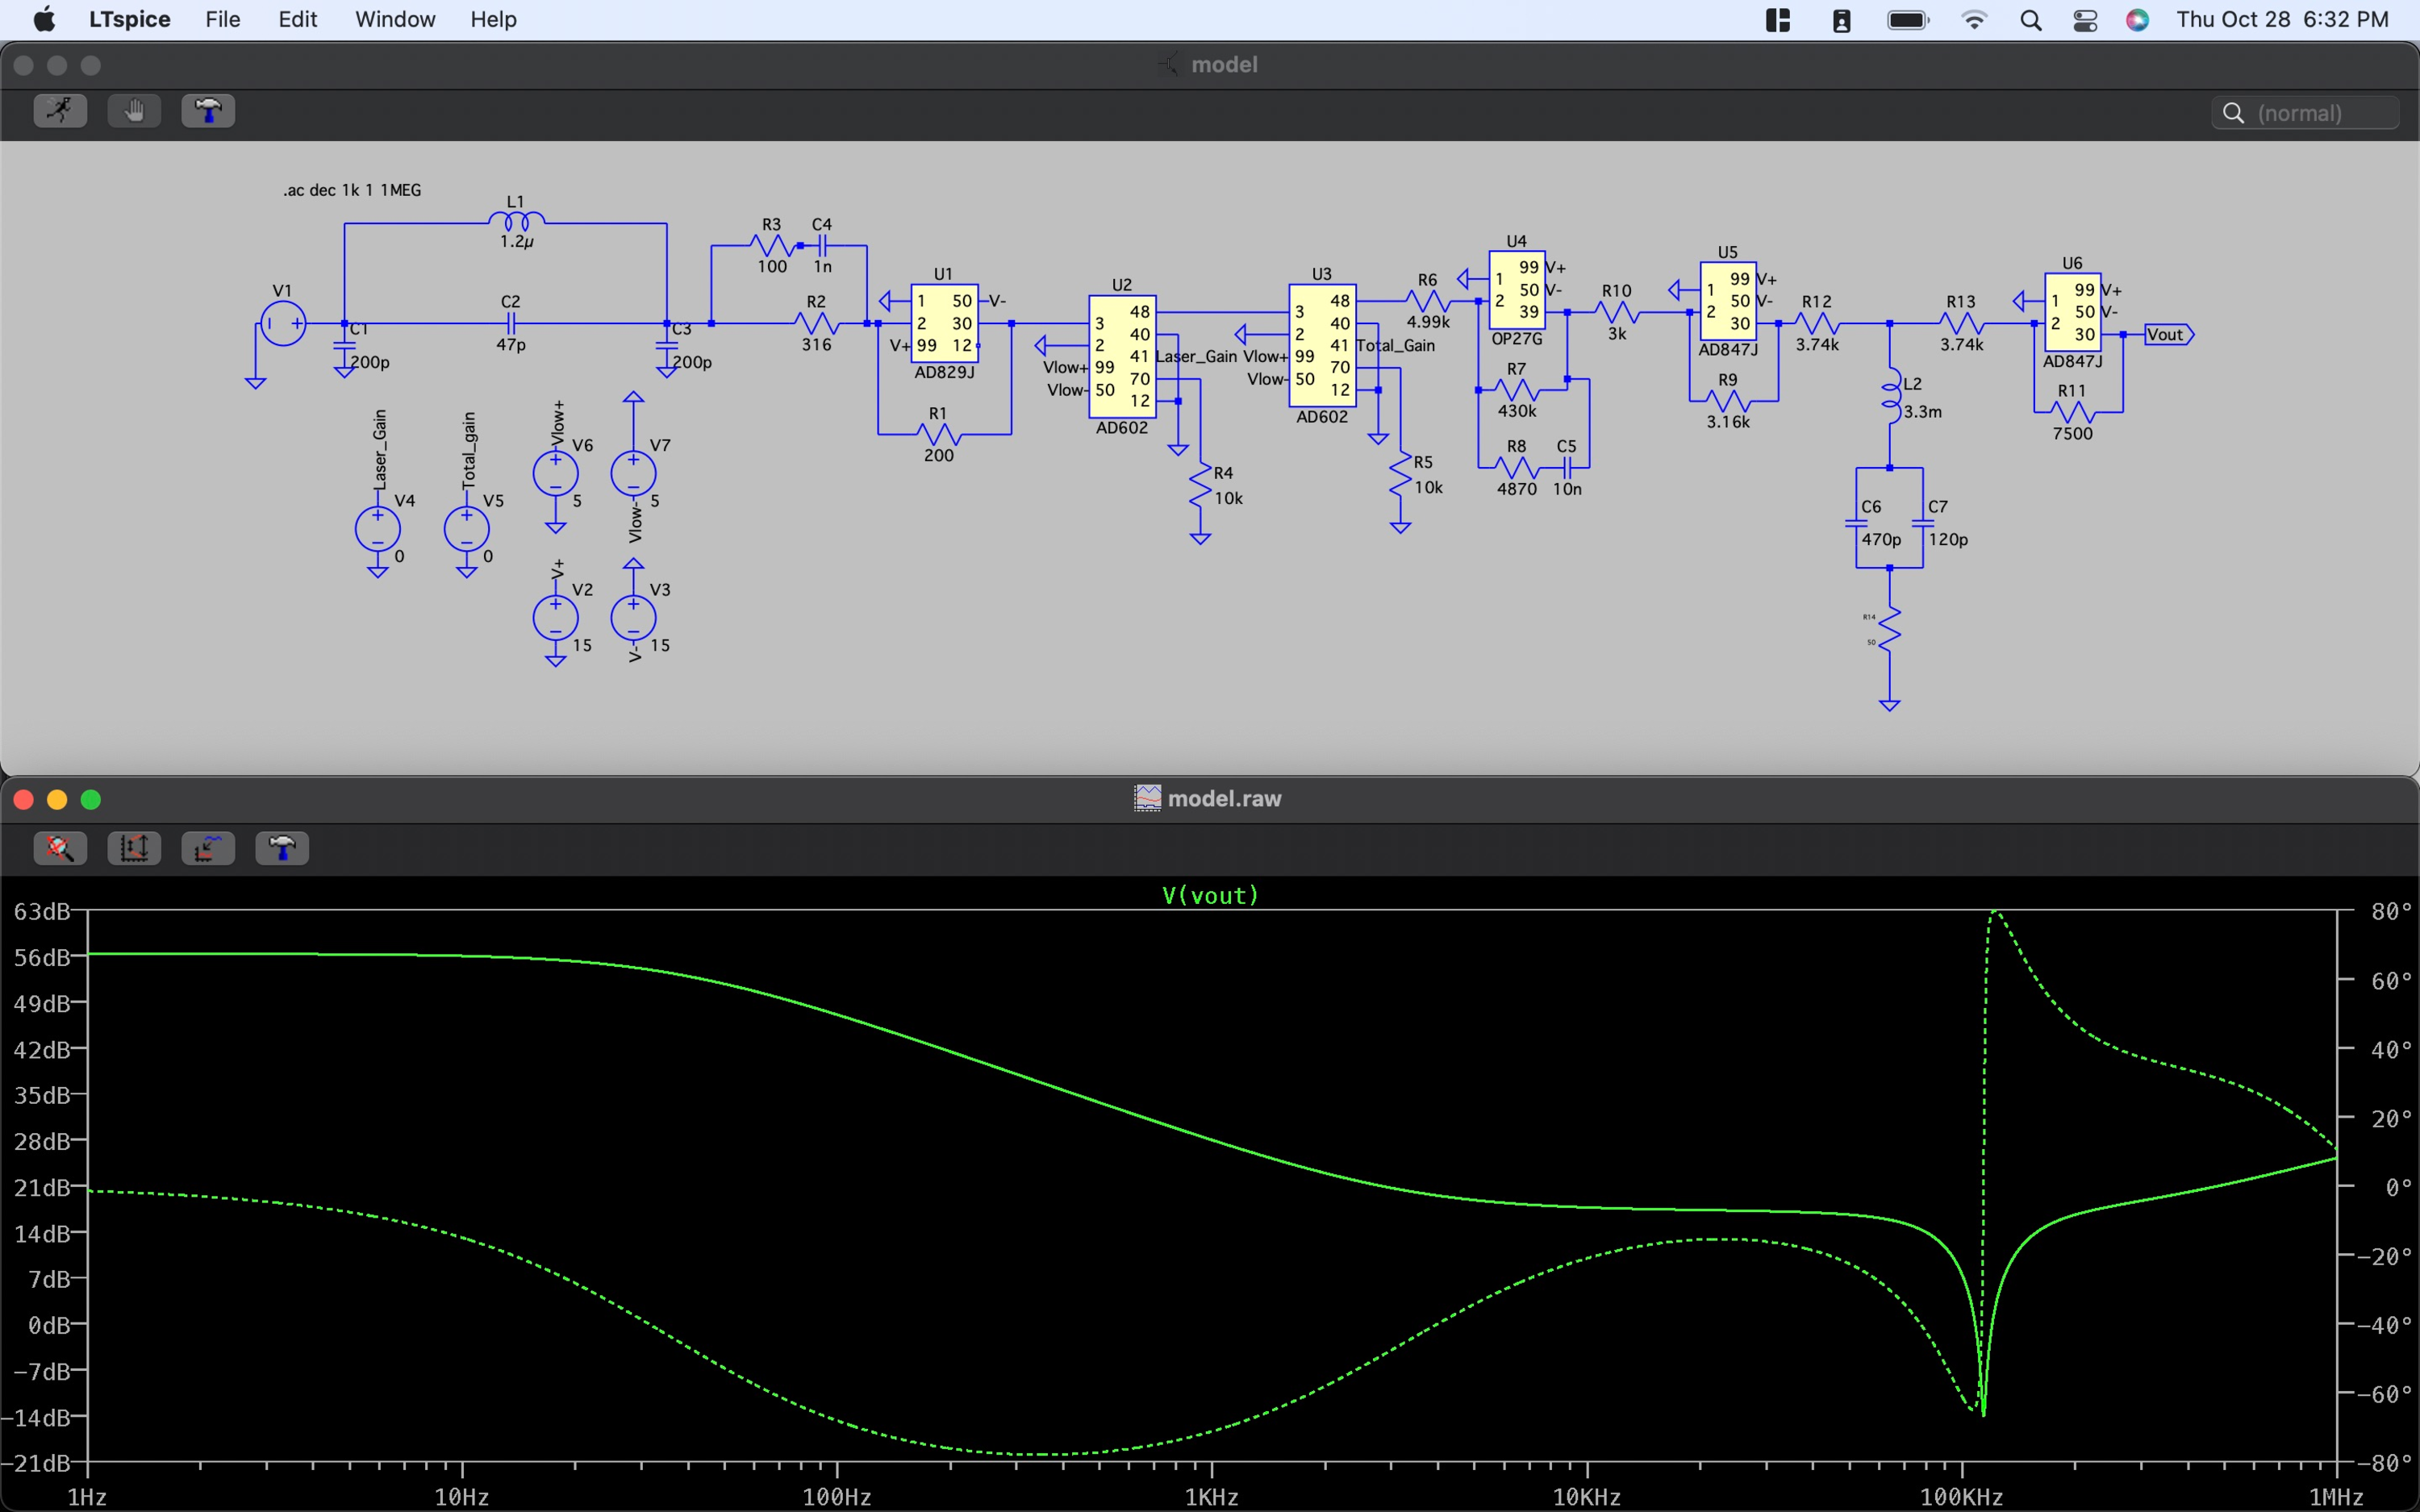
\includegraphics[width=\textwidth]{figs/ALGAAS/tfs/spice_FSS_tf.pdf}
    \caption{The FSS frequency response simulated in LTspice}
  \end{center}
  \label{fig:spiceFSS}
\end{figure}

\section{Measuring OLG [H]}

\begin{figure}[H]
  \begin{center}
    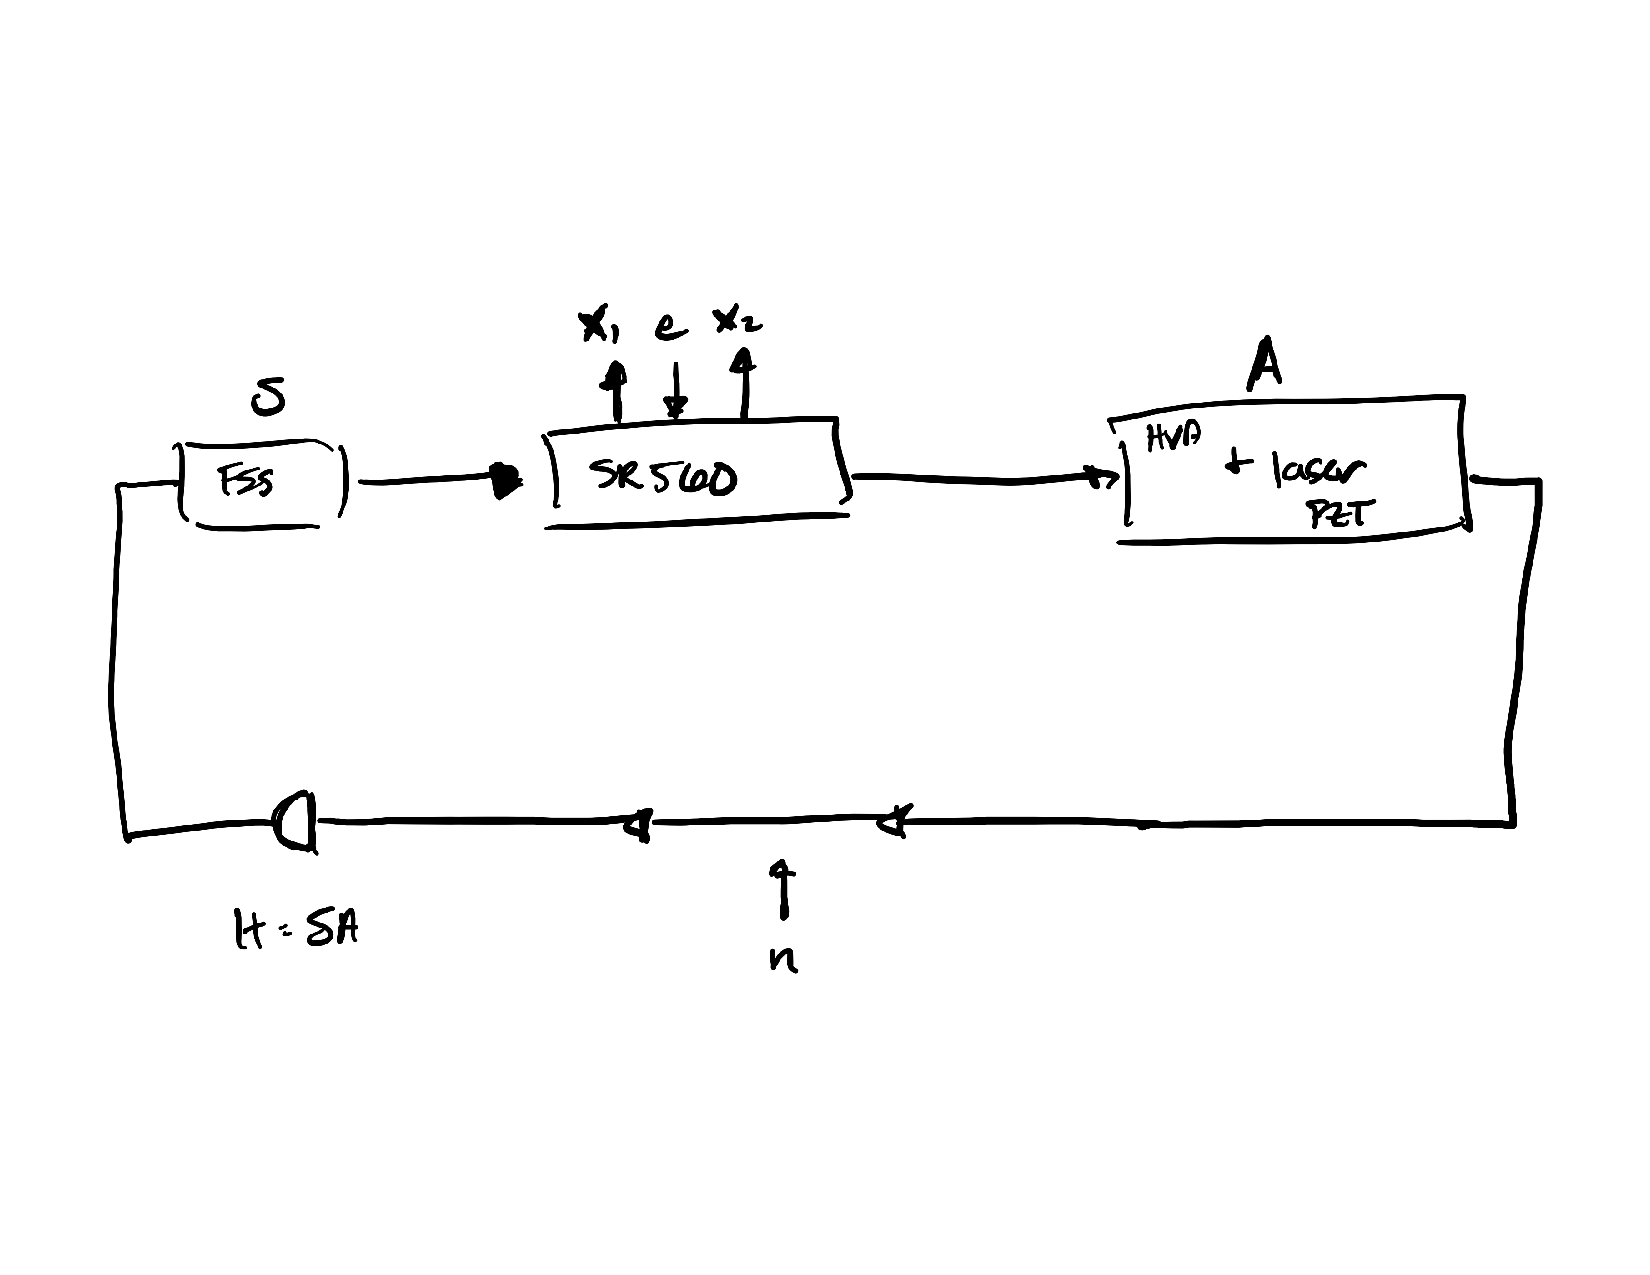
\includegraphics[width=.5\textwidth]{figs/ALGAAS/Loop_gain_measurement_drawn_diagram.pdf}
    \caption{Open loop gain measurement \textcolor{red}{drawn diagram}}
  \end{center}
  \label{fig:OLGmath}
\end{figure}

\textcolor{red}{x2 is the PSD taken immediately after the excitation point}
\begin{equation}
x_2 = e + He + H^2 e + \mathrm{H.O.T.s} = \frac{e + n}{1-H}
\end{equation}

\textcolor{red}{x1 is the PSD taken immediately prior to the excitation point}
\begin{equation}
x_1 = He + H^2e + H^3e + \mathrm{H.O.T.s}  = \frac{He}{1-H}
\end{equation}

We take the transfer function measurement $\zeta$:

\begin{equation}
\zeta = \frac{x_1}{x_2} = \frac{He/(1-H)}{(e+n)/(1-H)}
\end{equation}

Assuming the excitation is significantly larger than the noise ($e>>n$):

\begin{equation}
\zeta \approx H
\end{equation}
